%********************************************%
%*       Generated from PreTeXt source      *%
%*       on 2024-12-10T16:07:50-05:00       *%
%*   A recent stable commit (2022-07-01):   *%
%* 6c761d3dba23af92cba35001c852aac04ae99a5f *%
%*                                          *%
%*         https://pretextbook.org          *%
%*                                          *%
%********************************************%
\documentclass[twoside, 14pt]{extarticle}
%% Custom Preamble Entries, early (use latex.preamble.early)
%% Always open on odd page
%%   The following adjusts cleardoublepage to remove twosided
%%   check so that we open on odd pages even in one-sided mode
%%   by adding an extra blank page on the preceding even page.
\makeatletter%
\def\cleardoublepage{%
\clearpage\ifodd\c@page\else\thispagestyle{empty}\hbox{}\newpage\if@twocolumn\hbox{}\newpage\fi\fi%
}
\makeatother%
%% Default LaTeX packages
%%   1.  always employed (or nearly so) for some purpose, or
%%   2.  a stylewriter may assume their presence
\usepackage{geometry}
%% Some aspects of the preamble are conditional,
%% the LaTeX engine is one such determinant
\usepackage{ifthen}
%% etoolbox has a variety of modern conveniences
\usepackage{etoolbox}
\usepackage{ifxetex,ifluatex}
%% Raster graphics inclusion
\usepackage{graphicx}
%% Color support, xcolor package
%% Always loaded, for: add/delete text, author tools
%% Here, since tcolorbox loads tikz, and tikz loads xcolor
\PassOptionsToPackage{usenames,dvipsnames,svgnames,table}{xcolor}
\usepackage{xcolor}
%% begin: defined colors, via xcolor package, for styling
%% end: defined colors, via xcolor package, for styling
%% Colored boxes, and much more, though mostly styling
%% skins library provides "enhanced" skin, employing tikzpicture
%% boxes may be configured as "breakable" or "unbreakable"
%% "raster" controls grids of boxes, aka side-by-side
\usepackage{tcolorbox}
\tcbuselibrary{skins}
\tcbuselibrary{breakable}
\tcbuselibrary{raster}
%% We load some "stock" tcolorbox styles that we use a lot
%% Placement here is provisional, there will be some color work also
%% First, black on white, no border, transparent, but no assumption about titles
\tcbset{ bwminimalstyle/.style={enhanced, frame empty, extras broken={
          frame empty}, fonttitle=\bfseries, colback=white, colbacktitle=black!20, coltitle=black, opacityfill=1.0, } }
%% Second, bold title, run-in to text/paragraph/heading
%% Space afterwards will be controlled by environment,
%% independent of constructions of the tcb title
%% Places \blocktitlefont onto many block titles
\tcbset{ runintitlestyle/.style={fonttitle=\blocktitlefont\upshape\bfseries, attach title to upper} }
%% Spacing prior to each exercise, anywhere
\tcbset{ exercisespacingstyle/.style={before skip={1.5ex plus 0.5ex}} }
%% Spacing prior to each block
\tcbset{ blockspacingstyle/.style={before skip={2.0ex plus 0.5ex}} }
%% xparse allows the construction of more robust commands,
%% this is a necessity for isolating styling and behavior
%% The tcolorbox library of the same name loads the base library
\tcbuselibrary{xparse}
%% The tcolorbox library loads TikZ, its calc package is generally useful,
%% and is necessary for some smaller documents that use partial tcolor boxes
%% See:  https://github.com/PreTeXtBook/pretext/issues/1624
\usetikzlibrary{calc}
%% We use some more exotic tcolorbox keys to restore indentation to parboxes
\tcbuselibrary{hooks}
%% Save default paragraph indentation for use later, when adjusting parboxes
\newlength{\normalparindent}
\AtBeginDocument{\setlength{\normalparindent}{\parindent}}
%% Hyperref should be here, but likes to be loaded late
%%
%% Inline math delimiters, \(, \), need to be robust
%% 2016-01-31:  latexrelease.sty  supersedes  fixltx2e.sty
%% If  latexrelease.sty  exists, bugfix is in kernel
%% If not, bugfix is in  fixltx2e.sty
%% See:  https://tug.org/TUGboat/tb36-3/tb114ltnews22.pdf
%% and read "Fewer fragile commands" in distribution's  latexchanges.pdf
\IfFileExists{latexrelease.sty}{}{\usepackage{fixltx2e}}
%% shorter subnumbers in some side-by-side require manipulations
\usepackage{xstring}
%% Footnote counters and part/chapter counters are manipulated
%% April 2018:  chngcntr  commands now integrated into the kernel,
%% but circa 2018/2019 the package would still try to redefine them,
%% so we need to do the work of loading conditionally for old kernels.
%% From version 1.1a,  chngcntr  should detect defintions made by LaTeX kernel.
\ifdefined\counterwithin
\else
    \usepackage{chngcntr}
\fi
%% Text height identically 9 inches, text width varies on point size
%% See Bringhurst 2.1.1 on measure for recommendations
%% 75 characters per line (count spaces, punctuation) is target
%% which is the upper limit of Bringhurst's recommendations
\geometry{letterpaper, inner=1in, outer=0.7in, top=0.5in, bottom=0.7in}
%% Custom Page Layout Adjustments (use publisher page-geometry entry)
%% This LaTeX file may be compiled with pdflatex, xelatex, or lualatex executables
%% LuaTeX is not explicitly supported, but we do accept additions from knowledgeable users
%% The conditional below provides  pdflatex  specific configuration last
%% begin: engine-specific capabilities
\ifthenelse{\boolean{xetex} \or \boolean{luatex}}{%
%% begin: xelatex and lualatex-specific default configuration
\ifxetex\usepackage{xltxtra}\fi
%% realscripts is the only part of xltxtra relevant to lualatex 
\ifluatex\usepackage{realscripts}\fi
%% end:   xelatex and lualatex-specific default configuration
}{
%% begin: pdflatex-specific default configuration
%% We assume a PreTeXt XML source file may have Unicode characters
%% and so we ask LaTeX to parse a UTF-8 encoded file
%% This may work well for accented characters in Western language,
%% but not with Greek, Asian languages, etc.
%% When this is not good enough, switch to the  xelatex  engine
%% where Unicode is better supported (encouraged, even)
\usepackage[utf8]{inputenc}
%% end: pdflatex-specific default configuration
}
%% end:   engine-specific capabilities
%%
%% Fonts.  Conditional on LaTex engine employed.
%% Default Text Font: The Latin Modern fonts are
%% "enhanced versions of the [original TeX] Computer Modern fonts."
%% We use them as the default text font for PreTeXt output.
%% Default Monospace font: Inconsolata (aka zi4)
%% Sponsored by TUG: http://levien.com/type/myfonts/inconsolata.html
%% Loaded for documents with intentional objects requiring monospace
%% See package documentation for excellent instructions
%% fontspec will work universally if we use filename to locate OTF files
%% Loads the "upquote" package as needed, so we don't have to
%% Upright quotes might come from the  textcomp  package, which we also use
%% We employ the shapely \ell to match Google Font version
%% pdflatex: "varl" package option produces shapely \ell
%% pdflatex: "var0" package option produces plain zero (not used)
%% pdflatex: "varqu" package option produces best upright quotes
%% xelatex,lualatex: add OTF StylisticSet 1 for shapely \ell
%% xelatex,lualatex: add OTF StylisticSet 2 for plain zero (not used)
%% xelatex,lualatex: add OTF StylisticSet 3 for upright quotes
%%
%% Fancy Verbatim for consoles, preformatted, code display, literate programming
\usepackage{fancyvrb}
%% Pre-formatted text, a peer of paragraphs
\DefineVerbatimEnvironment{preformatted}{Verbatim}{}
%% Automatic Font Control
%% Portions of a document, are, or may, be affected by defined commands
%% These are perhaps more flexible when using  xelatex  rather than  pdflatex
%% The following definitions are meant to be re-defined in a style, using \renewcommand
%% They are scoped when employed (in a TeX group), and so should not be defined with an argument
\newcommand{\divisionfont}{\relax}
\newcommand{\blocktitlefont}{\relax}
\newcommand{\contentsfont}{\relax}
\newcommand{\pagefont}{\relax}
\newcommand{\tabularfont}{\relax}
\newcommand{\xreffont}{\relax}
\newcommand{\titlepagefont}{\relax}
%%
\ifthenelse{\boolean{xetex} \or \boolean{luatex}}{%
%% begin: font setup and configuration for use with xelatex
%% Generally, xelatex is necessary for non-Western fonts
%% fontspec package provides extensive control of system fonts,
%% meaning *.otf (OpenType), and apparently *.ttf (TrueType)
%% that live *outside* your TeX/MF tree, and are controlled by your *system*
%% (it is possible that a TeX distribution will place fonts in a system location)
%%
%% The fontspec package is the best vehicle for using different fonts in  xelatex
%% So we load it always, no matter what a publisher or style might want
%%
\usepackage{fontspec}
%%
%% begin: xelatex main font ("font-xelatex-main" template)
%% Latin Modern Roman is the default font for xelatex and so is loaded with a TU encoding
%% *in the format* so we can't touch it, only perhaps adjust it later
%% in one of two ways (then known by NFSS names such as "lmr")
%% (1) via NFSS with font family names such as "lmr" and "lmss"
%% (2) via fontspec with commands like \setmainfont{Latin Modern Roman}
%% The latter requires the font to be known at the system-level by its font name,
%% but will give access to OTF font features through optional arguments
%% https://tex.stackexchange.com/questions/470008/
%% where-and-how-does-fontspec-sty-specify-the-default-font-latin-modern-roman
%% http://tex.stackexchange.com/questions/115321
%% /how-to-optimize-latin-modern-font-with-xelatex
%%
%% end:   xelatex main font ("font-xelatex-main" template)
%% begin: xelatex mono font ("font-xelatex-mono" template)
%% (conditional on non-trivial uses being present in source)
\IfFontExistsTF{Inconsolatazi4-Regular.otf}{}{\GenericError{}{The font "Inconsolatazi4-Regular.otf" requested by PreTeXt output is not available.  Either a file cannot be located in default locations via a filename, or a font is not known by its name as part of your system.}{Consult the PreTeXt Guide for help with LaTeX fonts.}{}}
\IfFontExistsTF{Inconsolatazi4-Bold.otf}{}{\GenericError{}{The font "Inconsolatazi4-Bold.otf" requested by PreTeXt output is not available.  Either a file cannot be located in default locations via a filename, or a font is not known by its name as part of your system.}{Consult the PreTeXt Guide for help with LaTeX fonts.}{}}
\usepackage{zi4}
\setmonofont[BoldFont=Inconsolatazi4-Bold.otf,StylisticSet={1,3}]{Inconsolatazi4-Regular.otf}
%% end:   xelatex mono font ("font-xelatex-mono" template)
%% begin: xelatex font adjustments ("font-xelatex-style" template)
%% end:   xelatex font adjustments ("font-xelatex-style" template)
%%
%% Extensive support for other languages
\usepackage{polyglossia}
%% Set main/default language based on pretext/@xml:lang value
%% document language code is "es-ES", Spanish
\setmainlanguage{spanish}
%% Enable secondary languages based on discovery of @xml:lang values
%% Enable fonts/scripts based on discovery of @xml:lang values
%% Western languages should be ably covered by Latin Modern Roman
%% end:   font setup and configuration for use with xelatex
}{%
%% begin: font setup and configuration for use with pdflatex
%% begin: pdflatex main font ("font-pdflatex-main" template)
\usepackage{lmodern}
\usepackage[T1]{fontenc}
%% end:   pdflatex main font ("font-pdflatex-main" template)
%% begin: pdflatex mono font ("font-pdflatex-mono" template)
%% (conditional on non-trivial uses being present in source)
\usepackage[varqu,varl]{inconsolata}
%% end:   pdflatex mono font ("font-pdflatex-mono" template)
%% begin: pdflatex font adjustments ("font-pdflatex-style" template)
%% end:   pdflatex font adjustments ("font-pdflatex-style" template)
%% end:   font setup and configuration for use with pdflatex
}
%% Micromanage spacing, etc.  The named "microtype-options"
%% template may be employed to fine-tune package behavior
\usepackage{microtype}
%% Symbols, align environment, commutative diagrams, bracket-matrix
\usepackage{amsmath}
\usepackage{amscd}
\usepackage{amssymb}
%% allow page breaks within display mathematics anywhere
%% level 4 is maximally permissive
%% this is exactly the opposite of AMSmath package philosophy
%% there are per-display, and per-equation options to control this
%% split, aligned, gathered, and alignedat are not affected
\allowdisplaybreaks[4]
%% allow more columns to a matrix
%% can make this even bigger by overriding with  latex.preamble.late  processing option
\setcounter{MaxMatrixCols}{30}
%%
%%
%% Division Titles, and Page Headers/Footers
%% titlesec package, loading "titleps" package cooperatively
%% See code comments about the necessity and purpose of "explicit" option.
%% The "newparttoc" option causes a consistent entry for parts in the ToC 
%% file, but it is only effective if there is a \titleformat for \part.
%% "pagestyles" loads the  titleps  package cooperatively.
\usepackage[explicit, newparttoc, pagestyles]{titlesec}
%% The companion titletoc package for the ToC.
\usepackage{titletoc}
%% begin: customizations of page styles via the modal "titleps-style" template
%% Designed to use commands from the LaTeX "titleps" package
\pagestyle{plain}
%% end: customizations of page styles via the modal "titleps-style" template
%%
%% Create globally-available macros to be provided for style writers
%% These are redefined for each occurence of each division
%
% Number subsections ignoring sections
\renewcommand{\thesubsection}{\arabic{subsection}}
\makeatletter
\@removefromreset{subsection}{section}
\makeatother
%
%
\newcommand{\divisionnameptx}{\relax}%
\newcommand{\titleptx}{\relax}%
\newcommand{\subtitleptx}{\relax}%
\newcommand{\shortitleptx}{\relax}%
\newcommand{\authorsptx}{\relax}%
\newcommand{\epigraphptx}{\relax}%
%% Create environments for possible occurences of each division
%% Environment for a PTX "section" at the level of a LaTeX "section"
\NewDocumentEnvironment{sectionptx}{mmmmmmm}
{%
\renewcommand{\divisionnameptx}{#1}%
\renewcommand{\titleptx}{#2}%
\renewcommand{\subtitleptx}{#3}%
\renewcommand{\shortitleptx}{#4}%
\renewcommand{\authorsptx}{#5}%
\renewcommand{\epigraphptx}{#6}%
% \section{}%[{#4}]{#2}%
\label{#7}%
% \clearpage
}{}%
%% Environment for a PTX "subsection" at the level of a LaTeX "subsection"
\NewDocumentEnvironment{subsectionptx}{mmmmmmm}
{%
\renewcommand{\divisionnameptx}{#1}%
\renewcommand{\titleptx}{#2}%
\renewcommand{\subtitleptx}{#3}%
\renewcommand{\shortitleptx}{#4}%
\renewcommand{\authorsptx}{#5}%
\renewcommand{\epigraphptx}{#6}%
\vspace{-1.5cm}
\subsection{}%[{#4}]{#2}%
\label{#7}%
}{}%
%% Environment for a PTX "reading-questions" at the level of a LaTeX "subsubsection"
\NewDocumentEnvironment{reading-questions-subsubsection}{mmmmmmm}
{%
\renewcommand{\divisionnameptx}{#1}%
\renewcommand{\titleptx}{#2}%
\renewcommand{\subtitleptx}{#3}%
\renewcommand{\shortitleptx}{#4}%
\renewcommand{\authorsptx}{#5}%
\renewcommand{\epigraphptx}{#6}%
% \clearpage
\vspace{-0.4cm}
\subsubsection[{#4}]{Lección~\thesubsection~-~#2}%
\vspace{-0.4cm}
\label{#7}%
}{}%
%% Environment for a PTX "reading-questions" at the level of a LaTeX "subsubsection"
\NewDocumentEnvironment{reading-questions-subsubsection-numberless}{mmmmmmm}
{%
\renewcommand{\divisionnameptx}{#1}%
\renewcommand{\titleptx}{#2}%
\renewcommand{\subtitleptx}{#3}%
\renewcommand{\shortitleptx}{#4}%
\renewcommand{\authorsptx}{#5}%
\renewcommand{\epigraphptx}{#6}%
% \clearpage
\vspace{-1.2cm}
\subsubsection*{Lección~\thesubsection~-~#2}%
\vspace{-0.4cm}
\addcontentsline{toc}{subsubsection}{#4}
\label{#7}%
}{}%
%% Environment for a PTX "subsubsection" at the level of a LaTeX "subsubsection"
\NewDocumentEnvironment{subsubsectionptx}{mmmmmmm}
{%
\renewcommand{\divisionnameptx}{#1}%
\renewcommand{\titleptx}{#2}%
\renewcommand{\subtitleptx}{#3}%
\renewcommand{\shortitleptx}{#4}%
\renewcommand{\authorsptx}{#5}%
\renewcommand{\epigraphptx}{#6}%
% \clearpage
\vspace{-1.0cm}
\subsubsection[{#4}]{Lección~\thesubsection~-~#2}%
\vspace{-0.4cm}
\label{#7}%
}{}%
%% Environment for a PTX "exercises" at the level of a LaTeX "subsection"
\NewDocumentEnvironment{exercises-subsection}{mmmmmmm}
{%
\renewcommand{\divisionnameptx}{#1}%
\renewcommand{\titleptx}{#2}%
\renewcommand{\subtitleptx}{#3}%
\renewcommand{\shortitleptx}{#4}%
\renewcommand{\authorsptx}{#5}%
\renewcommand{\epigraphptx}{#6}%
\clearpage
\subsection*{#2}%
\label{#7}%
}{}%
%% Environment for a PTX "exercises" at the level of a LaTeX "subsection"
\NewDocumentEnvironment{exercises-subsection-numberless}{mmmmmmm}
{%
\renewcommand{\divisionnameptx}{#1}%
\renewcommand{\titleptx}{#2}%
\renewcommand{\subtitleptx}{#3}%
\renewcommand{\shortitleptx}{#4}%
\renewcommand{\authorsptx}{#5}%
\renewcommand{\epigraphptx}{#6}%
\subsection*{#2}%
\addcontentsline{toc}{subsection}{#4}
\label{#7}%
}{}%
%% Environment for a PTX "references" at the level of a LaTeX "subsection"
\NewDocumentEnvironment{references-subsection}{mmmmmmm}
{%
\renewcommand{\divisionnameptx}{#1}%
\renewcommand{\titleptx}{#2}%
\renewcommand{\subtitleptx}{#3}%
\renewcommand{\shortitleptx}{#4}%
\renewcommand{\authorsptx}{#5}%
\renewcommand{\epigraphptx}{#6}%
\subsection[{#4}]{Lección~\thesubsection - #2}%
\label{#7}%
}{}%
%% Environment for a PTX "references" at the level of a LaTeX "subsection"
\NewDocumentEnvironment{references-subsection-numberless}{mmmmmmm}
{%
\renewcommand{\divisionnameptx}{#1}%
\renewcommand{\titleptx}{#2}%
\renewcommand{\subtitleptx}{#3}%
\renewcommand{\shortitleptx}{#4}%
\renewcommand{\authorsptx}{#5}%
\renewcommand{\epigraphptx}{#6}%
\subsection*{#2}%
\addcontentsline{toc}{subsection}{Lección~\thesubsection - #4}
\label{#7}%
}{}%
%% Environment for a PTX "references" at the level of a LaTeX "section"
\NewDocumentEnvironment{references-section}{mmmmmmm}
{%
\renewcommand{\divisionnameptx}{#1}%
\renewcommand{\titleptx}{#2}%
\renewcommand{\subtitleptx}{#3}%
\renewcommand{\shortitleptx}{#4}%
\renewcommand{\authorsptx}{#5}%
\renewcommand{\epigraphptx}{#6}%
\section[{#4}]{#2}%
\label{#7}%
}{}%
%% Environment for a PTX "references" at the level of a LaTeX "section"
\NewDocumentEnvironment{references-section-numberless}{mmmmmmm}
{%
\renewcommand{\divisionnameptx}{#1}%
\renewcommand{\titleptx}{#2}%
\renewcommand{\subtitleptx}{#3}%
\renewcommand{\shortitleptx}{#4}%
\renewcommand{\authorsptx}{#5}%
\renewcommand{\epigraphptx}{#6}%
\section*{#2}%
\addcontentsline{toc}{section}{#4}
\label{#7}%
}{}%
%%
%% Styles for six traditional LaTeX divisions
\titleformat{\part}[display]
{\divisionfont\Huge\bfseries\centering}{\divisionnameptx\space\thepart}{30pt}{\Huge#1}
[{\Large\centering\authorsptx}]
\titleformat{\chapter}[display]
{\divisionfont\huge\bfseries}{\divisionnameptx\space\thechapter}{20pt}{\Huge#1}
[{\Large\authorsptx}]
\titleformat{name=\chapter,numberless}[display]
{\divisionfont\huge\bfseries}{}{0pt}{#1}
[{\Large\authorsptx}]
\titlespacing*{\chapter}{0pt}{50pt}{40pt}
\titleformat{\section}[hang]
{\divisionfont\Large\bfseries}{}{1ex}{#1}
[{\large\authorsptx}]
\titleformat{name=\section,numberless}[block]
{\divisionfont\Large\bfseries}{}{0pt}{#1}
[{\large\authorsptx}]
\titlespacing*{\section}{0pt}{3.5ex plus 1ex minus .2ex}{2.3ex plus .2ex}
\titleformat{\subsection}[hang]
{\divisionfont\large\bfseries}{}{1ex}{#1}
[{\normalsize\authorsptx}]
\titleformat{name=\subsection,numberless}[block]
{\divisionfont\large\bfseries}{}{0pt}{#1}
[{\normalsize\authorsptx}]
\titlespacing*{\subsection}{0pt}{3.25ex plus 1ex minus .2ex}{1.5ex plus .2ex}
\titleformat{\subsubsection}[hang]
{\divisionfont\normalsize\bfseries}{\thesubsubsection}{1em}{#1}
[{\small\authorsptx}]
\titleformat{name=\subsubsection,numberless}[block]
{\divisionfont\normalsize\bfseries}{}{0pt}{#1}
[{\normalsize\authorsptx}]
\titlespacing*{\subsubsection}{0pt}{3.25ex plus 1ex minus .2ex}{1.5ex plus .2ex}
\titleformat{\paragraph}[hang]
{\divisionfont\normalsize\bfseries}{\theparagraph}{1em}{#1}
[{\small\authorsptx}]
\titleformat{name=\paragraph,numberless}[block]
{\divisionfont\normalsize\bfseries}{}{0pt}{#1}
[{\normalsize\authorsptx}]
\titlespacing*{\paragraph}{0pt}{3.25ex plus 1ex minus .2ex}{1.5em}
%%
%% Styles for five traditional LaTeX divisions
\titlecontents{part}%
[0pt]{\contentsmargin{0em}\addvspace{1pc}\contentsfont\bfseries}%
{\Large\thecontentslabel\enspace}{\Large}%
{}%
[\addvspace{.5pc}]%
\titlecontents{chapter}%
[0pt]{\contentsmargin{0em}\addvspace{1pc}\contentsfont\bfseries}%
{\large\thecontentslabel\enspace}{\large}%
{\hfill\bfseries\thecontentspage}%
[\addvspace{.5pc}]%
\dottedcontents{section}[3.8em]{\contentsfont}{2.3em}{1pc}%
\dottedcontents{subsection}[6.1em]{\contentsfont}{3.2em}{1pc}%
\dottedcontents{subsubsection}[9.3em]{\contentsfont}{4.3em}{1pc}%
%%
%% Begin: Semantic Macros
%% To preserve meaning in a LaTeX file
%%
%% \mono macro for content of "c", "cd", "tag", etc elements
%% Also used automatically in other constructions
%% Simply an alias for \texttt
%% Always defined, even if there is no need, or if a specific tt font is not loaded
\newcommand{\mono}[1]{\texttt{#1}}
%%
%% Following semantic macros are only defined here if their
%% use is required only in this specific document
%%
%% Used for warnings, typically bold and italic
\newcommand{\alert}[1]{\textbf{\textit{#1}}}
%% Used for fillin answer blank in text
%% Relies on calc package, loaded via tcolorbox
%% Argument is intended number of characters of blank
%% Length may compress for output to fit in one line
\newlength{\fillinmaxwidth}
\newlength{\fillincontract}
\newlength{\fillinheight}
\newcommand{\fillintext}[1]{%
\setlength{\fillinmaxwidth}{#1em*\real{0.5}}%
\setlength{\fillincontract}{#1em*\real{0.5}*\real{0.2}}%
\setlength{\fillinheight}{\heightof{\strut}+1.2pt}%
\strut\nobreak\leaders\vbox{\hrule width 0.3pt height 0.3pt \vskip -1.2pt}\hskip 1\fillinmaxwidth minus \fillincontract\nobreak\strut%
}
%% End: Semantic Macros
%% Divisional exercises (and worksheet) as LaTeX environments
%% Third argument is option for extra workspace in worksheets
%% Hanging indent occupies a 5ex width slot prior to left margin
%% Experimentally this seems just barely sufficient for a bold "888."
%% Division exercises, not in exercise group
\tcbset{ divisionexercisestyle/.style={bwminimalstyle, runintitlestyle, exercisespacingstyle, left=2.3cm, breakable, before upper app={\setlength{\parskip}{\medskipamount}} } }
\newtcolorbox{divisionexercise}[4]{divisionexercisestyle, before title={\hspace{-5ex}\makebox[5ex][l]{#1.}}, title={\notblank{#2}{#2\space}{}}, phantom={\label{#4}\hypertarget{#4}{}}, after={}}
%% "tcolorbox" environment for a single image, occupying entire \linewidth
%% arguments are left-margin, width, right-margin, as multiples of
%% \linewidth, and are guaranteed to be positive and sum to 1.0
\tcbset{ imagestyle/.style={bwminimalstyle, blankest} }
\NewTColorBox{tcbimage}{mmm}{imagestyle}
%% Wrapper environment for tcbimage environment with a fourth argument
%% Fourth argument, if nonempty, is a vertical space adjustment
%% and implies image will be preceded by \leavevmode\nopagebreak
%% Intended use is for alignment with a list marker
\NewDocumentEnvironment{image}{mmmm}{\notblank{#4}{\leavevmode\nopagebreak\vspace{#4}}{~\par}\begin{tcbimage}{#1}{#2}{#3}}{\end{tcbimage}%
}%% For improved tables
\usepackage{array}
%% Some extra height on each row is desirable, especially with horizontal rules
%% Increment determined experimentally
\setlength{\extrarowheight}{0.2ex}
%% Define variable thickness horizontal rules, full and partial
%% Thicknesses are 0.03, 0.05, 0.08 in the  booktabs  package
\newcommand{\hrulethin}  {\noalign{\hrule height 0.04em}}
\newcommand{\hrulemedium}{\noalign{\hrule height 0.07em}}
\newcommand{\hrulethick} {\noalign{\hrule height 0.11em}}
%% We preserve a copy of the \setlength package before other
%% packages (extpfeil) get a chance to load packages that redefine it
\let\oldsetlength\setlength
\newlength{\Oldarrayrulewidth}
\newcommand{\crulethin}[1]%
{\noalign{\global\oldsetlength{\Oldarrayrulewidth}{\arrayrulewidth}}%
\noalign{\global\oldsetlength{\arrayrulewidth}{0.04em}}\cline{#1}%
\noalign{\global\oldsetlength{\arrayrulewidth}{\Oldarrayrulewidth}}}%
\newcommand{\crulemedium}[1]%
{\noalign{\global\oldsetlength{\Oldarrayrulewidth}{\arrayrulewidth}}%
\noalign{\global\oldsetlength{\arrayrulewidth}{0.07em}}\cline{#1}%
\noalign{\global\oldsetlength{\arrayrulewidth}{\Oldarrayrulewidth}}}
\newcommand{\crulethick}[1]%
{\noalign{\global\oldsetlength{\Oldarrayrulewidth}{\arrayrulewidth}}%
\noalign{\global\oldsetlength{\arrayrulewidth}{0.11em}}\cline{#1}%
\noalign{\global\oldsetlength{\arrayrulewidth}{\Oldarrayrulewidth}}}
%% Single letter column specifiers defined via array package
\newcolumntype{A}{!{\vrule width 0.04em}}
\newcolumntype{B}{!{\vrule width 0.07em}}
\newcolumntype{C}{!{\vrule width 0.11em}}
%% tcolorbox to place tabular outside of a sidebyside
\tcbset{ tabularboxstyle/.style={bwminimalstyle,} }
\newtcolorbox{tabularbox}[3]{tabularboxstyle, left skip=#1\linewidth, width=#2\linewidth,}
%% Footnote Numbering
%% Specified by numbering.footnotes.level
%% Global numbering, since numbering.footnotes.level = 0
%% Multiple column, column-major lists
\usepackage{multicol}
%% More flexible list management, esp. for references
%% But also for specifying labels (i.e. custom order) on nested lists
\usepackage{enumitem}
\setlist{nosep, topsep=0pt, partopsep=0.3ex, parsep=1ex}
%% Lists of references in their own section, maximum depth 1
\newlist{referencelist}{description}{4}
\setlist[referencelist]{leftmargin=!,labelwidth=!,labelsep=0ex,itemsep=1.0ex,topsep=1.0ex,partopsep=0pt,parsep=0pt}
%% Description lists as tcolorbox sidebyside
%% "dli" short for "description list item"
\newlength{\dlititlewidth}
\newlength{\dlimaxnarrowtitle}\setlength{\dlimaxnarrowtitle}{11ex}
\newlength{\dlimaxmediumtitle}\setlength{\dlimaxmediumtitle}{18ex}
\tcbset{ dlistyle/.style={sidebyside, sidebyside align=top seam, lower separated=false, bwminimalstyle, bottomtitle=0.75ex, after skip=1.5ex, boxsep=0pt, left=0pt, right=0pt, top=0pt, bottom=0pt} }
\tcbset{ dlinarrowstyle/.style={dlistyle, lefthand width=\dlimaxnarrowtitle, sidebyside gap=1ex, halign=flush left, righttitle=10ex} }
\tcbset{ dlimediumstyle/.style={dlistyle, lefthand width=\dlimaxmediumtitle, sidebyside gap=4ex, halign=flush right} }
\NewDocumentEnvironment{descriptionlist}{}{\par\vspace*{1.5ex}}{\par\vspace*{1.5ex}}%
%% begin enviroment has an if/then to open the tcolorbox
\NewDocumentEnvironment{dlinarrow}{mm}{%
\settowidth{\dlititlewidth}{{\textbf{#1}}}%
\ifthenelse{\dlititlewidth > \dlimaxnarrowtitle}%
{\begin{tcolorbox}[title={\textbf{#1}}, phantom={\hypertarget{#2}{}}, dlinarrowstyle]\tcblower}%
{\begin{tcolorbox}[dlinarrowstyle, phantom={\hypertarget{#2}{}}]\textbf{#1}\tcblower}%
}%
{\end{tcolorbox}}%
%% medium option is simpler
\NewDocumentEnvironment{dlimedium}{mm}%
{\begin{tcolorbox}[dlimediumstyle, phantom={\hypertarget{#2}{}}]\textbf{#1}\tcblower}%
{\end{tcolorbox}}%
%% hyperref driver does not need to be specified, it will be detected
%% Footnote marks in tcolorbox have broken linking under
%% hyperref, so it is necessary to turn off all linking
%% It *must* be given as a package option, not with \hypersetup
\usepackage[hyperfootnotes=false]{hyperref}
%% configure hyperref's  \href{}{}  and  \nolinkurl  to match listings' inline verbatim
\renewcommand\UrlFont{\small\ttfamily}
%% For a print PDF, no surrounding boxes, so simply textcolor (but still active to preserve spacing)
\hypersetup{hidelinks=true}
%% Less-clever names for hyperlinks are more reliable, *especially* for structural parts
%% See comments in the code to learn more about the importance of this setting
\hypersetup{hypertexnames=false}
%%The  hypertexnames  setting then confuses the hyperlinking from the index
%%This patch resolves the incorrect links, see code for StackExchange post.
\makeatletter
\patchcmd\Hy@EveryPageBoxHook{\Hy@EveryPageAnchor}{\Hy@hypertexnamestrue\Hy@EveryPageAnchor}{}{\fail}
\makeatother
\hypersetup{pdftitle={Matemáticas Ilustrativas}}
%% If you manually remove hyperref, leave in this next command
%% This will allow LaTeX compilation, employing this no-op command
\providecommand\phantomsection{}
%% Division Numbering: Chapters, Sections, Subsections, etc
%% Division numbers may be turned off at some level ("depth")
%% A section *always* has depth 1, contrary to us counting from the document root
%% The latex default is 3.  If a larger number is present here, then
%% removing this command may make some cross-references ambiguous
%% The precursor variable $numbering-maxlevel is checked for consistency in the common XSL file
\setcounter{secnumdepth}{2}
%%
%% AMS "proof" environment is no longer used, but we leave previously
%% implemented \qedhere in place, should the LaTeX be recycled
\newcommand{\qedhere}{\relax}
%%
%% A faux tcolorbox whose only purpose is to provide common numbering
%% facilities for most blocks (possibly not projects, 2D displays)
%% Controlled by  numbering.theorems.level  processing parameter
\newtcolorbox[auto counter]{block}{}
%%
%% This document is set to number PROJECT-LIKE on a separate numbering scheme
%% So, a faux tcolorbox whose only purpose is to provide this numbering
%% Controlled by  numbering.projects.level  processing parameter
\newtcolorbox[auto counter]{project-distinct}{}
%% A faux tcolorbox whose only purpose is to provide common numbering
%% facilities for 2D displays which are subnumbered as part of a "sidebyside"
\makeatletter
\newtcolorbox[auto counter, number within=tcb@cnt@block, number freestyle={\noexpand\thetcb@cnt@block(\noexpand\alph{\tcbcounter})}]{subdisplay}{}
\makeatother
%%
%% tcolorbox, with styles, for PROJECT-LIKE
%%
%% project: fairly simple numbered block/structure
\tcbset{ projectstyle/.style={bwminimalstyle, blockspacingstyle, before title={\vspace{0.3em}\strut}, after title={\strut\hfill Lección~\thesubsection \strut\vspace{0.15em}}, before upper app={\setlength{\parskip}{\medskipamount}}, } }
\newtcolorbox[use counter from=project-distinct]{project}[3]{title={#2}, phantomlabel={#3}, breakable, after={\par}, projectstyle, }
%% activity: fairly simple numbered block/structure
\tcbset{ activitystyle/.style={bwminimalstyle, blockspacingstyle, before title={\vspace{0.3em}}, after title={\strut\hfill Lección~\thesubsection \strut\vspace{0.15em}}, before upper app={\setlength{\parskip}{\medskipamount}}}, }
\newtcolorbox[use counter from=project-distinct]{activity}[3]{title={#2}, phantomlabel={#3}, breakable, after={\par}, activitystyle, }
%% exploration: fairly simple numbered block/structure
\tcbset{ explorationstyle/.style={bwminimalstyle, runintitlestyle, blockspacingstyle, after title={\space}, before upper app={\setlength{\parskip}{\medskipamount}}, } }
\newtcolorbox[use counter from=project-distinct]{exploration}[3]{title={{#1~\thetcbcounter\notblank{#2}{\space\space#2}{}}}, phantomlabel={#3}, breakable, after={\par}, explorationstyle, }
%%
%% xparse environments for introductions and conclusions of divisions
%%
%% introduction: in a structured division
\NewDocumentEnvironment{introduction}{m}
{\notblank{#1}{\noindent\textbf{#1}\space}{}}{\par\medskip}
%% paragraphs: the terminal, pseudo-division
%% We use the lowest LaTeX traditional division
\titleformat{\subparagraph}[runin]{\normalfont\normalsize\bfseries}{\thesubparagraph}{1em}{#1}
\titlespacing*{\subparagraph}{0pt}{3.25ex plus 1ex minus .2ex}{1em}
\NewDocumentEnvironment{paragraphs}{mm}
{\subparagraph*{#1}\label{#2}\hypertarget{#2}{}}{}
%% Graphics Preamble Entries
\usepackage{tikz, pgfplots}
\usetikzlibrary{positioning,matrix,arrows}
\usetikzlibrary{shapes,decorations,shadows,fadings,patterns}
\usetikzlibrary{decorations.markings}
%% If tikz has been loaded, replace ampersand with \amp macro
%% tcolorbox styles for sidebyside layout
\tcbset{ sbsstyle/.style={raster before skip=0.3ex, raster equal height=rows, raster force size=false, } }
\tcbset{ sbspanelstyle/.style={bwminimalstyle, fonttitle=\blocktitlefont, } }
%% Enviroments for side-by-side and components
%% Necessary to use \NewTColorBox for boxes of the panels
%% "newfloat" environment to squash page-breaks within a single sidebyside
%% "xparse" environment for entire sidebyside
\NewDocumentEnvironment{sidebyside}{mmmm}
  {\begin{tcbraster}
    [sbsstyle,raster columns=#1,
    raster left skip=#2\linewidth,raster right skip=#3\linewidth,raster column skip=#4\linewidth, ]}
  {\end{tcbraster}}
%% "tcolorbox" environment for a panel of sidebyside
\NewTColorBox{sbspanel}{mO{top}}{sbspanelstyle,width=#1\linewidth,valign=#2, }
%% Custom Preamble Entries, late (use latex.preamble.late)
%% extpfeil package for certain extensible arrows,
%% as also provided by MathJax extension of the same name
%% NB: this package loads mtools, which loads calc, which redefines
%%     \setlength, so it can be removed if it seems to be in the 
%%     way and your math does not use:
%%     
%%     \xtwoheadrightarrow, \xtwoheadleftarrow, \xmapsto, \xlongequal, \xtofrom
%%     
%%     we have had to be extra careful with variable thickness
%%     lines in tables, and so also load this package late
\usepackage{extpfeil}
%% Begin: Author-provided macros
%% (From  docinfo/macros  element)
%% Plus three from PTX for XML characters
\newcommand{\boldcdot}{\boldsymbol{\cdot}}
\newcommand{\unit}[1]{\,\text{#1}}
\newcommand{\lt}{<}
\newcommand{\gt}{>}
\newcommand{\amp}{&}
\usepackage[export]{adjustbox}% 'export' allows adjustbox keys in \includegraphics
% \renewcommand{\familydefault}{\sfdefault}
\usepackage[sfdefault]{roboto} 
\usepackage{sansmath}
\sansmath % Apply sansmath globally to all math environments
% \usepackage{microtype}
% stop hyphenation
\setlength{\emergencystretch}{3em}
\tolerance=1000
\hbadness=1000
\usepackage[none]{hyphenat} % Disable hyphenation
\hyphenpenalty=10000
\exhyphenpenalty=10000
% estilo de párrafos
\setlength{\parindent}{0pt}    % No indentation for new paragraphs
\setlength{\parskip}{1ex}     % Small space between paragraphs 
% Quitar justificación (lineas igual de anchas)
\usepackage[document]{ragged2e}
% headers y footers
\usepackage{fancyhdr}
\pagestyle{fancy}
\fancyfoot[C]{} %Remove default Latex numbering
\fancyhead[C]{\begin{tikzpicture}[remember picture,overlay] \node[yshift=-0.5cm] at (current page.north west) {\begin{tikzpicture}[remember picture, overlay] 
\includegraphics[width=\paperwidth]{external/cools-pdf/barra-colorGrupoLEMA.png}\end{tikzpicture}};\end{tikzpicture}} % Paper-Wide header
% \fancyfoot[C]{{\small Grupo LEMA (www.grupolema.org), \the\year{}. Licencia de uso CC-BY-NC Internacional 4.0.}\\{\scriptsize Adaptado de IM K–5 Math v.I, © 2021 Illustrative Mathematics ® illustrativemathematics.org en su versión en español en im.kendallhunt.com y de Open Up Resources © 2022, openupresources.org, publicadas bajo una licencia Creative Commons CC BY 4.0. Detalles: https://creativecommons.org/licenses/by/4.0/deed.es}}
\fancyhead[L]{}%{\rightmark}
\fancyhead[R]{}
% \fancyfoot[R]{}
\fancyfoot[RO, LE]{\textcolor{PineGreen}{\textbf{\thepage}}}
\fancyfoot[C]{\small Libro de trabajo}%{\rightmark}
\fancyfootoffset{1cm} % Set offsets for header/footer closer to the edge
\fancypagestyle{plain}{}  % Redefine the plain page style (style used in title pages)
% \renewcommand{\footrulewidth}{1pt}  % Agregar linea all footer
\renewcommand{\headrulewidth}{0pt}  % Quitar linea del header
%% End: Author-provided macros
%% Title page information for article
\title{Matemáticas Ilustrativas\\
{\large Grado 3 - Unidad 4}\\[1ex]{\Huge Libro de trabajo}}
\author{Adaptación del Grupo LEMA\\
\href{https://www.grupolema.org}{\nolinkurl{https://www.grupolema.org}}
}
% Custom abstract environment for smaller text and smaller footnotes
\makeatletter
\renewenvironment{abstract}{%
    \small\par\noindent\textbf{\abstractname}\par\noindent
    \footnotesize % Make abstract text smaller
    \let\old@footnotesize\footnotesize % Save original footnotesize
    % \renewcommand{\footnotesize}{\tiny} % Make footnotes in abstract smaller  
    \renewcommand{\UrlFont}{\footnotesize\ttfamily} % Make \url and \nolinkurl tiny and typewriter font
    % \quotation
}{%
    % \endquotation
    \let\footnotesize\old@footnotesize % Restore original footnotesize
    \renewcommand{\UrlFont}{\ttfamily} % Restore default \UrlFont
}
\makeatother
\date{December 10, 2024}
\begin{document}
%% bottom alignment is explicit, since it normally depends on oneside, twoside
\raggedbottom
%% Target for xref to top-level element is document start
\label{gra3-uni4}\hypertarget{gra3-uni4}{}
\maketitle
\thispagestyle{empty}
\renewcommand*{\abstractname}{}
\begin{abstract}
Este documento (HTML, pdf, latex o epub) se generó con \href{https://pretextbook.org}{PreTeXt}\footnote{\nolinkurl{pretextbook.org}\label{meta-source-2-2}}. El código fuente con el contenido para generarlo se encuentra en \href{https://github.com/enriqueacosta/IllustrativeMath-GrupoLEMA}{\nolinkurl{github.com/enriqueacosta}}.%
\end{abstract}
\clearpage
\renewcommand*{\abstractname}{Licencia}
\begin{abstract}
2024~Versión PreTeXt, traducciones completas de las guías y adaptaciones © Enrique Acosta (\href{https://enriqueacosta.github.io}{\nolinkurl{enriqueacosta.github.io}}). Iniciativa del Grupo LEMA (\href{https://www.grupolema.org}{\nolinkurl{www.grupolema.org}})Publicado bajo una licencia Creative Commons Attribution-NonCommercial-ShareAlike 4.0 International (CC BY SA NC 4.0).%
\par
En breve e incompleto (los detalles están en las licencias), \alert{tiene toda libertad para adaptar, copiar y distribuir este material siempre y cuando le mantenga la misma licencia, incluya la atribución correspondiente (mencione a Enrique Acosta, al Grupo LEMA, a Illustrative Mathematics y a OpenUp Resources en la forma que se describe a continuación) y lo use para fines no comerciales}.%
\par
Ver detalles de la licencia en \href{https://creativecommons.org/licenses/by-nc-sa/4.0/}{creativecommons.org}\footnote{\nolinkurl{creativecommons.org/licenses/by-nc-sa/4.0/}\label{meta-copyright-6-2}}.%
\par
Además, se permite la impresión y distribución a costo para uso educativo o personal. La reventa comercial o actividades con fines de lucro no están permitidas sin autorización previa.%
\par
Grados K-5 adaptados de IM K–5 Math v.I, ©~2021 Illustrative Mathematics~® \href{https://curriculum.illustrativemathematics.org}{illustrativemathematics.org}\footnote{\nolinkurl{curriculum.illustrativemathematics.org}\label{meta-copyright-8-4}} en su versión en español en \href{https://im.kendallhunt.com/K5_ES/curriculum.html}{im.kendallhunt.com}\footnote{\nolinkurl{im.kendallhunt.com/K5_ES/curriculum.html}\label{meta-copyright-8-6}}, distribuido con una licencia Creative Commons Attribution 4.0 International License (CC BY 4.0). Ver detalles de esta licencia en \href{https://creativecommons.org/licenses/by/4.0/}{creativecommons.org}\footnote{\nolinkurl{creativecommons.org/licenses/by/4.0/}\label{meta-copyright-8-8}}.%
\par
Grados 6-8 adaptados de IM 6–8 v3.1415, ©~2019 Illustrative Mathematics~® \href{https://curriculum.illustrativemathematics.org}{illustrativemathematics.org}\footnote{\nolinkurl{curriculum.illustrativemathematics.org}\label{meta-copyright-9-4}} en su versión en español en \href{https://im.kendallhunt.com/K5_ES/curriculum.html}{im.kendallhunt.com}\footnote{\nolinkurl{im.kendallhunt.com/K5_ES/curriculum.html}\label{meta-copyright-9-6}}, distribuido con una licencia Creative Commons Attribution 4.0 International License (CC BY 4.0), a su vez ©~2017-2019 Open Up Resources 6–8 Math v2, disponibles en \href{https://openupresources.org/math-curriculum/}{openupresources.org}\footnote{\nolinkurl{openupresources.org/math-curriculum/}\label{meta-copyright-9-9}}, con la misma licencia (CC BY 4.0). Ver detalles de esta licencia en \href{https://creativecommons.org/licenses/by/4.0/}{creativecommons.org}\footnote{\nolinkurl{creativecommons.org/licenses/by/4.0/}\label{meta-copyright-9-11}}.%
\par
\alert{Nota:} Las traducciones anteriormente mencionadas fueron lideradas y coordinadas por miembros del Grupo LEMA. Ver detalles en:%
\begin{itemize}[label=\textbullet]
\item{}K-5: \href{https://curriculum.illustrativemathematics.org/k5/teachers/grade-1/course-guide/contributors.html}{illustrativemathematics.org}\footnote{\nolinkurl{curriculum.illustrativemathematics.org/k5/teachers/grade-1/course-guide/contributors.html}\label{meta-copyright-10-2-1-2}}%
\item{}6-8: \href{https://curriculum.illustrativemathematics.org/MS/teachers/1/contributors.html}{illustrativemathematics.org}\footnote{\nolinkurl{curriculum.illustrativemathematics.org/MS/teachers/1/contributors.html}\label{meta-copyright-10-2-2-2}}%
\item{}\href{https://enriqueacosta.github.io/blog/es/posts/translating-im/}{enriqueacosta.github.io}\footnote{\nolinkurl{enriqueacosta.github.io/blog/es/posts/translating-im/}\label{meta-copyright-10-2-3-2}}%
\end{itemize}
%
\par
Este material incluye imágenes con licencias abiertas que tiene copyright de sus respectivos autores. Estas imágenes mantienen los términos de sus propias licencias de uso. Ver detalles en la sección de atribuciones de imágenes.%
\end{abstract}
%
\clearpage
\renewcommand*{\abstractname}{Gracias a ...}
\begin{abstract}
Las siguientes personas aportaron en el desarrollo de esta versión de Matemáticas Ilustrativas.%
\par
Traducción y procesamiento de contenido%
%
\begin{itemize}[label=\textbullet]
\item{}Enrique Acosta Jaramillo%
\item{}Andrés Forero Cuervo%
\item{}Nathaly Otero Paternina%
\item{}Jonathan Defelipe Payane%
\end{itemize}
Ingeniería y desarrollo%
%
\begin{itemize}[label=\textbullet]
\item{}Enrique Acosta Jaramillo%
\end{itemize}
Autores (en inglés)%
%
\begin{itemize}[label=\textbullet]
\item{}Illustrative Mathematics. Ver detalles en los siguientes enlaces.%
%
\begin{itemize}[label=$\circ$]
\item{}K-5: \href{https://im.kendallhunt.com/k5_es/teachers/grade-4/course-guide/contributors.html}{https:\slash{}\slash{}im.kendallhunt.com\slash{}k5\slash{}}\footnote{\nolinkurl{im.kendallhunt.com/k5_es/teachers/grade-4/course-guide/contributors.html}\label{meta-contributors-8-1-2-1-2}}%
\item{}6-8: \href{https://im.kendallhunt.com/MS/teachers/2/contributors.html}{https:\slash{}\slash{}im.kendallhunt.com\slash{}MS\slash{}}\footnote{\nolinkurl{im.kendallhunt.com/MS/teachers/2/contributors.html}\label{meta-contributors-8-1-2-2-2}}%
\end{itemize}
\end{itemize}
\end{abstract}
\renewcommand*{\abstractname}{y gracias a ...}
\begin{abstract}
Los distintos formatos de este documento (PDF, LaTeX, EPUB) se generaron utilizando software de licencia abierta desarrollado gracias al esfuerzo de muchas personas. Entre estos destacamos:%
%
\begin{itemize}[label=\textbullet]
\item{}\href{https://pretextbook.org}{Pretext}\footnote{\nolinkurl{pretextbook.org}\label{meta-attributionsOpenSource-3-1-2}}: Sistema para crear y publicar libros de texto, artículos de investigación y monografías, especialmente en disciplinas STEM.%
\item{}\href{https://www.mathjax.org}{MathJax}\footnote{\nolinkurl{www.mathjax.org}\label{meta-attributionsOpenSource-3-2-2}}: Biblioteca JavaScript para mostrar fórmulas matemáticas en cualquier navegador web.%
\item{}\href{https://www.latex-project.org}{LaTeX}\footnote{\nolinkurl{www.latex-project.org}\label{meta-attributionsOpenSource-3-3-2}} y \href{https://tug.org}{TeX}\footnote{\nolinkurl{tug.org}\label{meta-attributionsOpenSource-3-3-4}}: Sistema de preparación de documentos para impresión, ampliamente usado para documentos profesionales.%
\item{}\href{https://ctan.org/pkg/pgf}{TikZ}\footnote{\nolinkurl{ctan.org/pkg/pgf}\label{meta-attributionsOpenSource-3-4-2}}: Paquete de LaTeX para crear gráficos vectoriales de alta calidad, desde diagramas matemáticos hasta ilustraciones técnicas y científicas.%
\item{}\href{https://ctan.org/pkg/fontawesome}{FontAwesome}\footnote{\nolinkurl{ctan.org/pkg/fontawesome}\label{meta-attributionsOpenSource-3-5-2}}: Iconos vectoriales y herramientas de diseño para LaTeX.%
\end{itemize}
\end{abstract}
%
%
\typeout{************************************************}
\typeout{Sección  Sección A -~¿Qué es la división?}
\typeout{************************************************}
%
\cleardoublepage
\begin{sectionptx}{Sección}{Sección A -~¿Qué es la división?}{}{Sección A -~¿Qué es la división?}{}{}{gra3-uni4-secA}
\newpage
%
%
\typeout{************************************************}
\typeout{Subsección  Lección 1 -~¿Cuántos grupos?}
\typeout{************************************************}
%
\begin{subsectionptx}{Subsección}{Lección 1 -~¿Cuántos grupos?}{}{Lección 1}{}{}{lec-cuantosGrupos}
%
%
\typeout{************************************************}
\typeout{Preguntas de comprensión  Actividad de cierre}
\typeout{************************************************}
%
\begin{reading-questions-subsubsection-numberless}{Preguntas de comprensión}{Actividad de cierre}{}{Actividad de cierre}{}{}{lec-cuantosGrupos-cool}
\begin{project}{Actividad de cierre}{¿Cuántas bolsas?}{cool-cuantasBolsas}%
Lin tiene 30 manzanas para compartirlas con sus amigos. Las pone en bolsas y pone 6 manzanas en cada bolsa. ¿Cuántas bolsas necesita? Explica o muestra tu razonamiento.%
\begin{image}{0}{1}{0}{}%

\includegraphics[max width=\linewidth, center]{external/whitespace-tikz/4cm.pdf}
\end{image}%
\end{project}%
\end{reading-questions-subsubsection-numberless}
\end{subsectionptx}
%
%
\typeout{************************************************}
\typeout{Subsección  Lección 2 -~¿Cuántos hay en cada grupo?}
\typeout{************************************************}
%
\begin{subsectionptx}{Subsección}{Lección 2 -~¿Cuántos hay en cada grupo?}{}{Lección 2}{}{}{lec-cuantosEnCadaGrupo}
%
%
\typeout{************************************************}
\typeout{Preguntas de comprensión  Actividad de cierre}
\typeout{************************************************}
%
\begin{reading-questions-subsubsection-numberless}{Preguntas de comprensión}{Actividad de cierre}{}{Actividad de cierre}{}{}{lec-cuantosEnCadaGrupo-cool}
\begin{project}{Actividad de cierre}{Bolsas de manzanas.}{cool-bolsasManzanas}%
Lin tiene 30 manzanas. Ella prepara 6 bolsas con el mismo número de manzanas en cada bolsa para dárselas a sus amigos. ¿Cuántas manzanas hay en cada bolsa? Explica o muestra tu razonamiento.%
\begin{image}{0}{1}{0}{}%

\includegraphics[max width=\linewidth, center]{external/whitespace-tikz/4cm.pdf}
\end{image}%
\end{project}%
\end{reading-questions-subsubsection-numberless}
\end{subsectionptx}
%
%
\typeout{************************************************}
\typeout{Subsección  Lección 3 -~Dibujos de situaciones de división}
\typeout{************************************************}
%
\begin{subsectionptx}{Subsección}{Lección 3 -~Dibujos de situaciones de división}{}{Lección 3}{}{}{lec-dibujosSituacionesDivision}
%
%
\typeout{************************************************}
\typeout{Preguntas de comprensión  Actividad de cierre}
\typeout{************************************************}
%
\clearpage
\begin{reading-questions-subsubsection-numberless}{Preguntas de comprensión}{Actividad de cierre}{}{Actividad de cierre}{}{}{lec-dibujosSituacionesDivision-cool}
\begin{project}{Actividad de cierre}{Regalitos para invitados.}{cool-regalitosInvitados}%
Clare tiene 48 marcadores. Ella pone 8 marcadores en cada bolsa de regalitos para su fiesta de cumpleaños. ¿Cuántas bolsas usará?%
\par
¿Cuál dibujo corresponde a la situación? Explica tu razonamiento.%
\begin{sidebyside}{2}{0}{0}{0}%
\begin{sbspanel}{0.5}%
A.%
\par
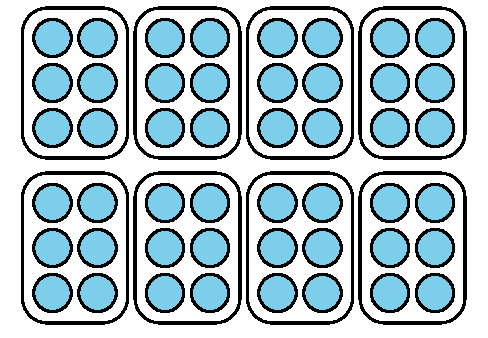
\includegraphics[max width=\linewidth, center]{external/svg-source/tikz-file-246306.pdf}
\end{sbspanel}%
\begin{sbspanel}{0.5}%
B.%
\par
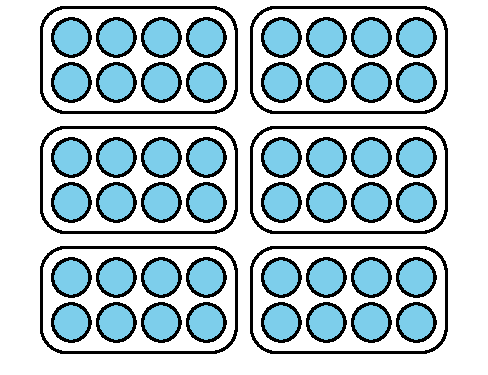
\includegraphics[max width=\linewidth, center]{external/svg-source/tikz-file-246307.pdf}
\end{sbspanel}%
\end{sidebyside}%
\begin{image}{0}{1}{0}{}%

\includegraphics[max width=\linewidth, center]{external/whitespace-tikz/2cm.pdf}
\end{image}%
\end{project}%
\end{reading-questions-subsubsection-numberless}
\end{subsectionptx}
%
%
\typeout{************************************************}
\typeout{Subsección  Lección 4 -~Interpretemos expresiones de división}
\typeout{************************************************}
%
\begin{subsectionptx}{Subsección}{Lección 4 -~Interpretemos expresiones de división}{}{Lección 4}{}{}{lec-interpretarExpresionesDivision}
%
%
\typeout{************************************************}
\typeout{Preguntas de comprensión  Actividad de cierre}
\typeout{************************************************}
%
\begin{reading-questions-subsubsection-numberless}{Preguntas de comprensión}{Actividad de cierre}{}{Actividad de cierre}{}{}{lec-interpretarExpresionesDivision-cool}
\begin{project}{Actividad de cierre}{Los trompos de Han.}{cool-losTromposDe}%
Han tiene 14 trompos. Él reparte los trompos equitativamente en 2 cajas. ¿Cuántos trompos habrá en cada caja?%
\par
Selecciona \alert{todas} las formas en las que podemos representar la situación.%
\begin{sidebyside}{4}{0.0075}{0.0075}{0.015}%
\begin{sbspanel}{0.04}%
A%
\end{sbspanel}%
\begin{sbspanel}{0.45}%
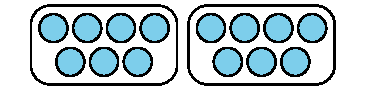
\includegraphics[max width=\linewidth, center]{external/svg-source/tikz-file-151100.pdf}
\end{sbspanel}%
\begin{sbspanel}{0.04}%
B%
\end{sbspanel}%
\begin{sbspanel}{0.45}%
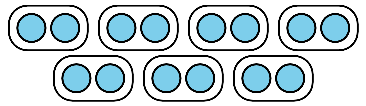
\includegraphics[max width=\linewidth, center]{external/svg-source/tikz-file-151101.pdf}
\end{sbspanel}%
\end{sidebyside}%
\begin{sidebyside}{4}{0.0075}{0.0075}{0.015}%
\begin{sbspanel}{0.04}%
C%
\end{sbspanel}%
\begin{sbspanel}{0.45}%
\par
%
\begin{equation*}
14\div 2
\end{equation*}
%
\end{sbspanel}%
\begin{sbspanel}{0.04}%
\par
D%
\end{sbspanel}%
\begin{sbspanel}{0.45}%
\par
%
\begin{equation*}
14\div 7
\end{equation*}
%
\end{sbspanel}%
\end{sidebyside}%
\end{project}%
\end{reading-questions-subsubsection-numberless}
\end{subsectionptx}
%
%
\typeout{************************************************}
\typeout{Subsección  Lección 5 -~Escribamos expresiones de división}
\typeout{************************************************}
%
\begin{subsectionptx}{Subsección}{Lección 5 -~Escribamos expresiones de división}{}{Lección 5}{}{}{lec-escribamosExpresionesDivision}
%
%
\typeout{************************************************}
\typeout{Subsubsección  Actividad 1}
\typeout{************************************************}
%
\begin{subsubsectionptx}{Subsubsección}{Actividad 1}{}{Actividad 1}{}{}{lec-escribamosExpresionesDivision-act1}
\begin{activity}{Actividad}{Clasificación de tarjetas: Todo sobre bichos.}{act-clasificacionDeTarjetas-todoSobreBichos}%
%
\begin{enumerate}
\item{}Tu profesor te dará un grupo de tarjetas que muestran situaciones. Elige dos categorías y clasifica las tarjetas en esas dos categorías. Prepárate para explicar el significado de tus categorías.%
\item{}Escribe una expresión de división para representar cada situación. Prepárate para explicar tu razonamiento.%
%
\begin{enumerate}[label={\Alph*.}]
\item{}\begin{image}{0}{1}{0}{-1.5\baselineskip}%

\includegraphics[max width=\linewidth, center]{external/whitespace-tikz/2cm.pdf}
\end{image}%
%
\item{}\begin{image}{0}{1}{0}{-1.5\baselineskip}%

\includegraphics[max width=\linewidth, center]{external/whitespace-tikz/2cm.pdf}
\end{image}%
%
\item{}\begin{image}{0}{1}{0}{-1.5\baselineskip}%

\includegraphics[max width=\linewidth, center]{external/whitespace-tikz/2cm.pdf}
\end{image}%
%
\item{}\begin{image}{0}{1}{0}{-1.5\baselineskip}%

\includegraphics[max width=\linewidth, center]{external/whitespace-tikz/2cm.pdf}
\end{image}%
%
\item{}\begin{image}{0}{1}{0}{-1.5\baselineskip}%

\includegraphics[max width=\linewidth, center]{external/whitespace-tikz/2cm.pdf}
\end{image}%
%
\item{}\begin{image}{0}{1}{0}{-1.5\baselineskip}%

\includegraphics[max width=\linewidth, center]{external/whitespace-tikz/2cm.pdf}
\end{image}%
%
\end{enumerate}
\end{enumerate}
\end{activity}%
\cleardoublepage
Tarjetas para recortar:%
\par
\begin{image}{0}{1}{0}{1cm}%
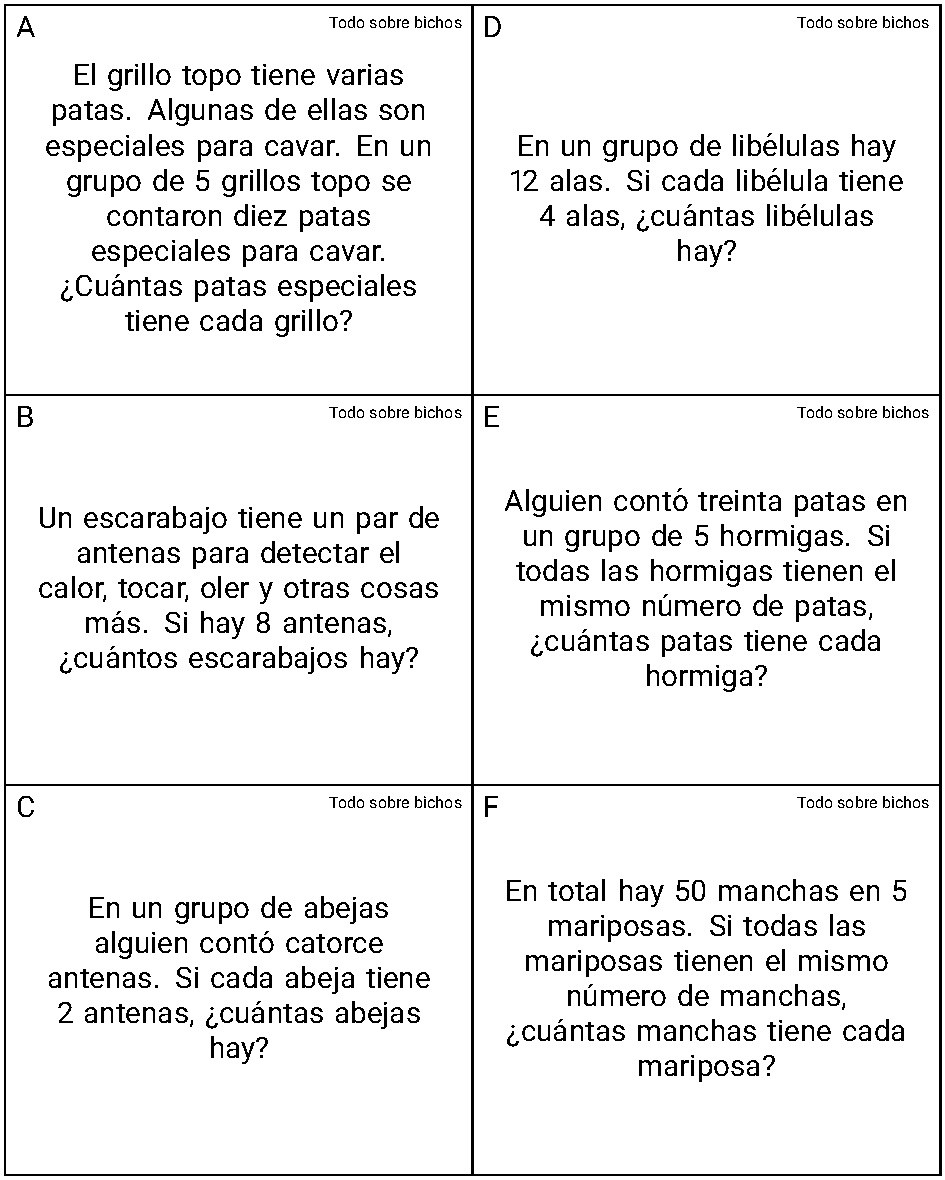
\includegraphics[max width=\linewidth, center]{external/tikz-source/todoSobreBichos-tarjetas.pdf}
\end{image}%
\cleardoublepage
\end{subsubsectionptx}
%
%
\typeout{************************************************}
\typeout{Preguntas de comprensión  Actividad de cierre}
\typeout{************************************************}
%
\clearpage
\begin{reading-questions-subsubsection}{Preguntas de comprensión}{Actividad de cierre}{}{Actividad de cierre}{}{}{lec-escribamosExpresionesDivision-cool}
\begin{project}{Actividad de cierre}{Patas de hormigas.}{cool-patasHormigas}%
Veinticuatro patas pertenecen a 4 hormigas. Todas las hormigas tienen el mismo número de patas.%
\par
%
\begin{enumerate}[label={(\alph*)}]
\item{}Escribe una expresión de división que represente esta situación.%
\begin{image}{0}{1}{0}{}%

\includegraphics[max width=\linewidth, center]{external/whitespace-tikz/2cm.pdf}
\end{image}%
\item{}¿Cuántas patas tiene cada hormiga? Explica o muestra tu razonamiento.%
\begin{image}{0}{1}{0}{}%

\includegraphics[max width=\linewidth, center]{external/whitespace-tikz/4cm.pdf}
\end{image}%
\end{enumerate}
%
\end{project}%
\end{reading-questions-subsubsection}
\end{subsectionptx}
%
%
\typeout{************************************************}
\typeout{Ejercicios  Problemas de práctica de la sección A}
\typeout{************************************************}
%
\begin{exercises-subsection}{Ejercicios}{Problemas de práctica de la sección A}{}{Problemas de práctica}{}{}{gra3-uni4-secA-ProblemasPractica}
\begin{divisionexercise}{1}{(Previo a la sección).}{}{gra3-uni4-secA-ProblemasPractica-3}%
\begin{sidebyside}{2}{0}{0}{0}%
\begin{sbspanel}{0.3}[top]%
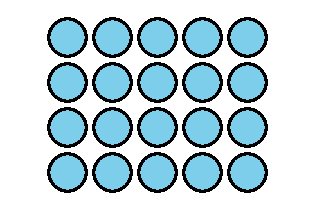
\includegraphics[max width=\linewidth, center]{external/svg-source/tikz-file-151668.pdf}
\end{sbspanel}%
\begin{sbspanel}{0.7}[top]%
%
\begin{enumerate}[label={(\alph*)}]
\item{}Escribe una expresión de multiplicación que represente el arreglo.%
\par

\includegraphics[max width=\linewidth, center]{external/whitespace-tikz/1cm.pdf}
\item{}Escribe una ecuación de multiplicación que represente el arreglo.%
\par

\includegraphics[max width=\linewidth, center]{external/whitespace-tikz/1cm.pdf}
\end{enumerate}
%
\end{sbspanel}%
\end{sidebyside}%
\end{divisionexercise}%
\begin{divisionexercise}{2}{(Previo a la sección).}{}{gra3-uni4-secA-ProblemasPractica-4}%
Encuentra el área de cada rectángulo.%
\begin{sidebyside}{2}{0.05}{0.05}{0.1}%
\begin{sbspanel}{0.3}%
A.%
\par
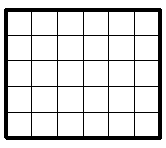
\includegraphics[max width=\linewidth, center]{external/svg-source/tikz-file-151669-scale13.pdf}
\end{sbspanel}%
\begin{sbspanel}{0.5}%
B.%
\par
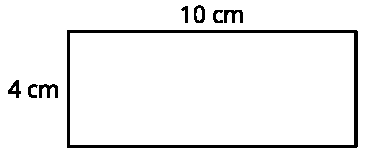
\includegraphics[max width=\linewidth, center]{external/svg-source/tikz-file-151670-scale13.pdf}
\end{sbspanel}%
\end{sidebyside}%
\begin{image}{0}{1}{0}{}%

\includegraphics[max width=\linewidth, center]{external/whitespace-tikz/1cm.pdf}
\end{image}%
\end{divisionexercise}%
\begin{divisionexercise}{3}{(Previo a la sección).}{}{gra3-uni4-secA-ProblemasPractica-5}%
El área del rectángulo es 40 centímetros cuadrados.%
\begin{sidebyside}{2}{0}{0}{0}%
\begin{sbspanel}{0.5}[top]%
Encuentra la longitud de lado desconocida del rectángulo. Explica tu razonamiento.%
\end{sbspanel}%
\begin{sbspanel}{0.5}[top]%
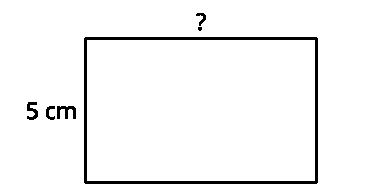
\includegraphics[max width=\linewidth, center]{external/svg-source/tikz-file-151673-scale13.pdf}
\end{sbspanel}%
\end{sidebyside}%
% \begin{image}{0}{1}{0}{}%
% 
\includegraphics[max width=\linewidth, center]{external/whitespace-tikz/4cm.pdf}
% \end{image}%
\end{divisionexercise}%
\begin{divisionexercise}{4}{(Previo a la sección).}{}{gra3-uni4-secA-ProblemasPractica-6}%
En cada caso, encuentra el número que hace que la ecuación sea verdadera.%
\par
%
\begin{enumerate}[label={(\alph*)}]
\item{}\(\displaystyle 8 \times 5 = \underline{\hspace{1cm}}\)%
\item{}\(\displaystyle 5 \times \underline{\hspace{1cm}} = 35\)%
\item{}\(\displaystyle \underline{\hspace{1cm}} \times 2 = 18\)%
\end{enumerate}
%
\end{divisionexercise}%
\begin{divisionexercise}{5}{(Previo a la sección).}{}{gra3-uni4-secA-ProblemasPractica-7}%
Hay 6 equipos de voleibol en el gimnasio. Cada equipo tiene 10 jugadores. ¿Cuántos jugadores de voleibol hay en total?%
\par
%
\begin{enumerate}[label={(\alph*)}]
\item{}Haz un dibujo de la situación.%
\begin{image}{0}{1}{0}{}%

\includegraphics[max width=\linewidth, center]{external/whitespace-tikz/4cm.pdf}
\end{image}%
\item{}Escribe una ecuación que represente la situación. Usa un “?” para representar el valor desconocido.%
\begin{image}{0}{1}{0}{}%

\includegraphics[max width=\linewidth, center]{external/whitespace-tikz/3cm.pdf}
\end{image}%
\item{}Resuelve el problema.%
\begin{image}{0}{1}{0}{}%

\includegraphics[max width=\linewidth, center]{external/whitespace-tikz/4cm.pdf}
\end{image}%
\end{enumerate}
%
\end{divisionexercise}%
\clearpage
\begin{divisionexercise}{6}{}{}{gra3-uni4-secA-ProblemasPractica-8}%
En cada problema, usa un dibujo o un diagrama para mostrar cómo pensaste.%
\par
%
\begin{enumerate}[label={(\alph*)}]
\item{}Hay 40 manzanas empacadas en cajas. Si hay 8 manzanas en cada caja, ¿cuántas cajas hay?%
\begin{image}{0}{1}{0}{}%

\includegraphics[max width=\linewidth, center]{external/whitespace-tikz/3cm.pdf}
\end{image}%
\item{}Hay 40 manzanas empacadas en cajas. Si hay 10 manzanas en cada caja, ¿cuántas cajas hay?%
\begin{image}{0}{1}{0}{}%

\includegraphics[max width=\linewidth, center]{external/whitespace-tikz/3cm.pdf}
\end{image}%
\end{enumerate}
%
\end{divisionexercise}%
\begin{divisionexercise}{7}{}{}{gra3-uni4-secA-ProblemasPractica-9}%
En cada problema, usa un dibujo o un diagrama para mostrar cómo pensaste.%
%
\begin{enumerate}[label={(\alph*)}]
\item{}Hay 30 naranjas. Si se empacan en 5 bolsas con la misma cantidad de naranjas en cada bolsa, ¿cuántas naranjas hay en cada bolsa?%
\begin{image}{0}{1}{0}{}%

\includegraphics[max width=\linewidth, center]{external/whitespace-tikz/3cm.pdf}
\end{image}%
\item{}Hay 30 naranjas. Si se empacan en 3 bolsas con la misma cantidad de naranjas en cada bolsa, ¿cuántas naranjas hay en cada bolsa?%
\begin{image}{0}{1}{0}{}%

\includegraphics[max width=\linewidth, center]{external/whitespace-tikz/3cm.pdf}
\end{image}%
\end{enumerate}
\end{divisionexercise}%
\begin{divisionexercise}{8}{}{}{gra3-uni4-secA-ProblemasPractica-10}%
%
\vspace{-2.8ex}
\begin{enumerate}[label={(\alph*)}]
\item{}10 personas van a cine en automóviles. En cada automóvil van dos personas. ¿Cuántos automóviles hay? Muestra cómo pensaste. Usa un dibujo o un diagrama.%
\begin{image}{0}{1}{0}{}%

\includegraphics[max width=\linewidth, center]{external/whitespace-tikz/4cm.pdf}
\end{image}%
\item{}Otras 10 personas van a cine en automóviles. Van en 2 automóviles con el mismo número de personas en cada automóvil. ¿Cuántas personas hay en cada automóvil? Muestra cómo pensaste. Usa un dibujo o un diagrama.%
\begin{image}{0}{1}{0}{}%

\includegraphics[max width=\linewidth, center]{external/whitespace-tikz/4cm.pdf}
\end{image}%
\item{}¿En qué se parecen las dos situaciones? ¿En qué son diferentes? ¿En qué se parecen los diagramas? ¿En qué son diferentes?%
\begin{image}{0}{1}{0}{}%

\includegraphics[max width=\linewidth, center]{external/whitespace-tikz/3cm.pdf}
\end{image}%
\end{enumerate}
%
\end{divisionexercise}%
\clearpage
\begin{divisionexercise}{9}{}{}{gra3-uni4-secA-ProblemasPractica-11}%
Hay 20 pupitres en la clase. Están divididos equitativamente en 5 grupos. ¿Cuántos pupitres hay en cada grupo?%
\par
%
\begin{enumerate}[label={(\alph*)}]
\item{}¿Cuál expresión representa esta situación: \(20\div 4\) o \(20\div 5\)? Explica tu razonamiento.%
\begin{image}{0}{1}{0}{}%

\includegraphics[max width=\linewidth, center]{external/whitespace-tikz/1cm.pdf}
\end{image}%
\item{}Selecciona el diagrama que representa esta situación. Explica tu razonamiento.%
\begin{sidebyside}{2}{0}{0}{0}%
\begin{sbspanel}{0.06}%
A%
\end{sbspanel}%
\begin{sbspanel}{0.95}%
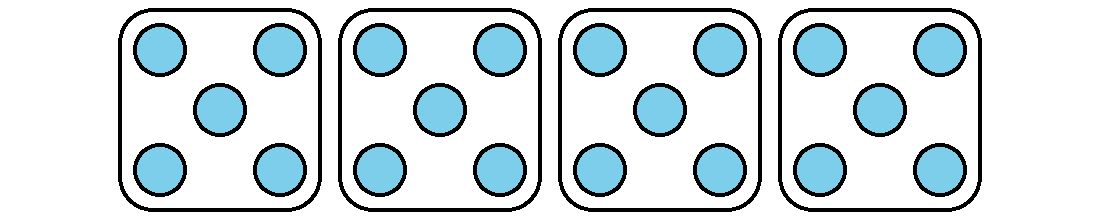
\includegraphics[max width=\linewidth, center]{external/svg-source/tikz-file-151671.pdf}
\end{sbspanel}%
\end{sidebyside}%
\begin{sidebyside}{2}{0}{0}{0}%
\begin{sbspanel}{0.06}%
B%
\end{sbspanel}%
\begin{sbspanel}{0.95}%

\includegraphics[max width=\linewidth, center]{external/svg-source/tikz-file-151672.pdf}
\end{sbspanel}%
\end{sidebyside}%
\begin{image}{0}{1}{0}{}%

\includegraphics[max width=\linewidth, center]{external/whitespace-tikz/2cm.pdf}
\end{image}%
\end{enumerate}
%
\end{divisionexercise}%
\begin{divisionexercise}{10}{}{}{gra3-uni4-secA-ProblemasPractica-12}%
La familia de Mai recolectó 40 libras de duraznos y los pusieron en bolsas. Pusieron 5 libras en cada bolsa.%
\par
%
\begin{enumerate}[label={(\alph*)}]
\item{}Escribe una expresión de división que represente la situación.%
\begin{image}{0}{1}{0}{}%

\includegraphics[max width=\linewidth, center]{external/whitespace-tikz/1cm.pdf}
\end{image}%
\item{}¿Cuántas bolsas de duraznos recogió la familia de Mai? Explica o muestra tu razonamiento.%
\begin{image}{0}{1}{0}{}%

\includegraphics[max width=\linewidth, center]{external/whitespace-tikz/3cm.pdf}
\end{image}%
\end{enumerate}
%
\end{divisionexercise}%
\begin{divisionexercise}{11}{Exploración.}{}{gra3-uni4-secA-ProblemasPractica-13}%
Completa cada historia poniendo un número que tenga sentido en el espacio en blanco. Después, responde las preguntas. Dibuja un diagrama para resolver cada problema.%
\par
%
\begin{enumerate}[label={(\alph*)}]
\item{}Mai tiene \textunderscore{}\textunderscore{}\textunderscore{}\textunderscore{}\textunderscore{}\textunderscore{}\textunderscore{}\textunderscore{}\textunderscore{}\textunderscore{} calcomanías. Ella va a poner el mismo número de calcomanías en cada uno de sus 5 cuadernos. ¿Cuántas calcomanías habrá en cada cuaderno?%
\begin{image}{0}{1}{0}{}%

\includegraphics[max width=\linewidth, center]{external/whitespace-tikz/4cm.pdf}
\end{image}%
\item{}Andre tiene \textunderscore{}\textunderscore{}\textunderscore{}\textunderscore{}\textunderscore{}\textunderscore{}\textunderscore{}\textunderscore{}\textunderscore{}\textunderscore{} tarjetas. Él va a organizarlas en filas de \textunderscore{}\textunderscore{}\textunderscore{}\textunderscore{}\textunderscore{}\textunderscore{}\textunderscore{}\textunderscore{}\textunderscore{}\textunderscore{} tarjetas. ¿Cuántas filas de tarjetas hará Andre?%
\begin{image}{0}{1}{0}{}%

\includegraphics[max width=\linewidth, center]{external/whitespace-tikz/4cm.pdf}
\end{image}%
\end{enumerate}
%
\end{divisionexercise}%
\begin{divisionexercise}{12}{Exploración.}{}{gra3-uni4-secA-ProblemasPractica-14}%
Escribe una situación de división que corresponda a cada diagrama.%
\begin{sidebyside}{3}{0}{0}{0.02}%
\begin{sbspanel}{0.32}%
A%
\par
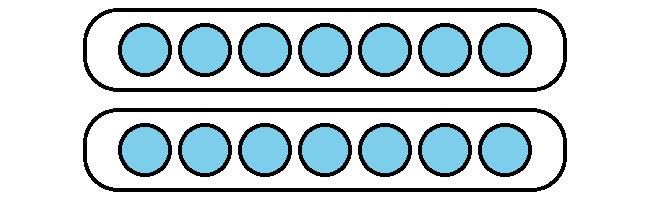
\includegraphics[max width=\linewidth, center]{external/svg-source/tikz-file-151674.pdf}
\end{sbspanel}%
\begin{sbspanel}{0.32}%
B%
\par
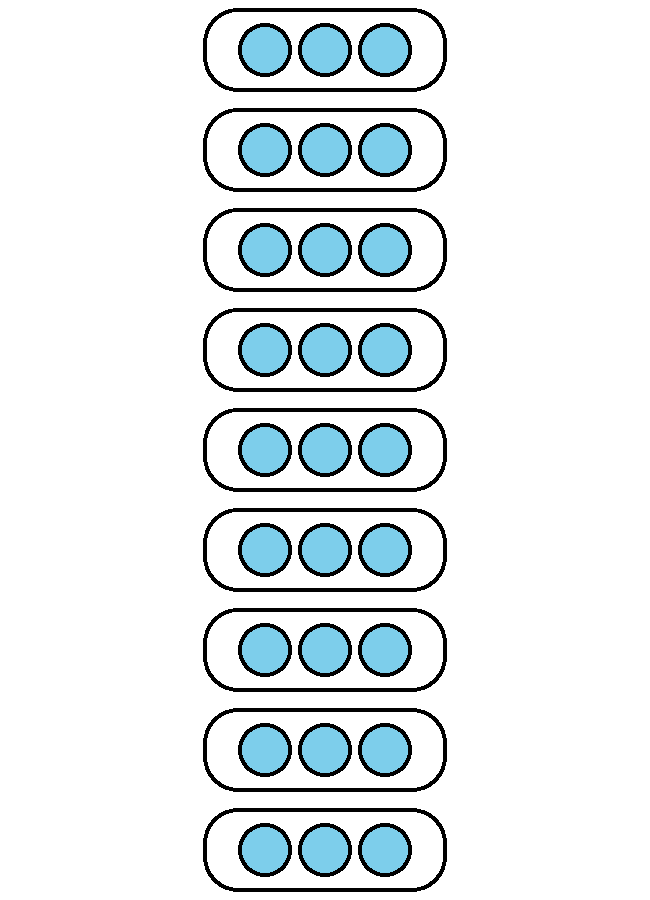
\includegraphics[max width=\linewidth, center]{external/svg-source/tikz-file-151675.pdf}
\end{sbspanel}%
\begin{sbspanel}{0.32}%
C%
\par
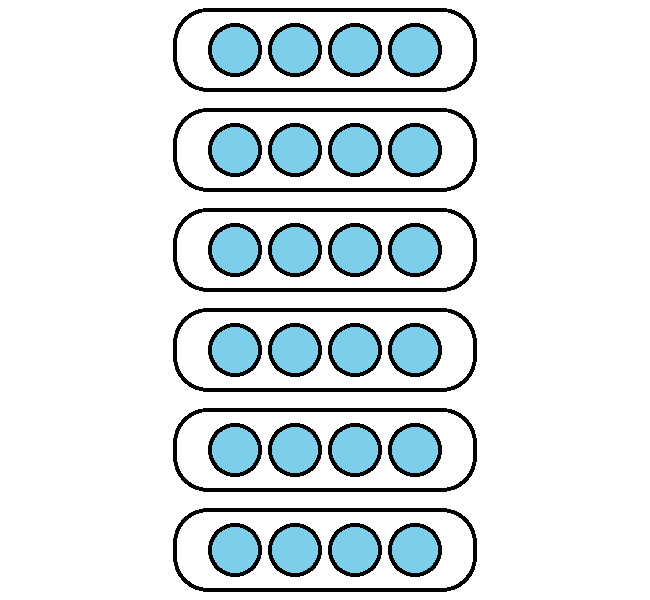
\includegraphics[max width=\linewidth, center]{external/svg-source/tikz-file-151676.pdf}
\end{sbspanel}%
\end{sidebyside}%
% \begin{image}{0}{1}{0}{}%
% 
\includegraphics[max width=\linewidth, center]{external/whitespace-tikz/1cm.pdf}
% \end{image}%
\end{divisionexercise}%
\end{exercises-subsection}
\end{sectionptx}
%
%
\typeout{************************************************}
\typeout{Sección  Sección B -~Relacionemos la multiplicación y la división}
\typeout{************************************************}
%
% \begin{sectionptx}{Sección}{Sección B -~Relacionemos la multiplicación y la división}{}{Sección B -~Relacionemos la multiplicación y la división}{}{}{gra3-uni4-secB}
%
%
\typeout{************************************************}
\typeout{Subsección  Lección 6 -~La división como un factor desconocido}
\typeout{************************************************}
%
\begin{subsectionptx}{Subsección}{Lección 6 -~La división como un factor desconocido}{}{Lección 6}{}{}{lec-divisionComoFactorDesconocido}
%
%
\typeout{************************************************}
\typeout{Subsubsección  Actividad 2}
\typeout{************************************************}
%
\begin{subsubsectionptx}{Subsubsección}{Actividad 2}{}{Actividad 2}{}{}{lec-divisionComoFactorDesconocido-act2}
\begin{activity}{Actividad}{En el mercado agrícola.}{act-enElMercadoAgricola}%
Completa cada fila. Prepárate para explicar tu razonamiento.%
\begin{image}{0}{1}{0}{}%
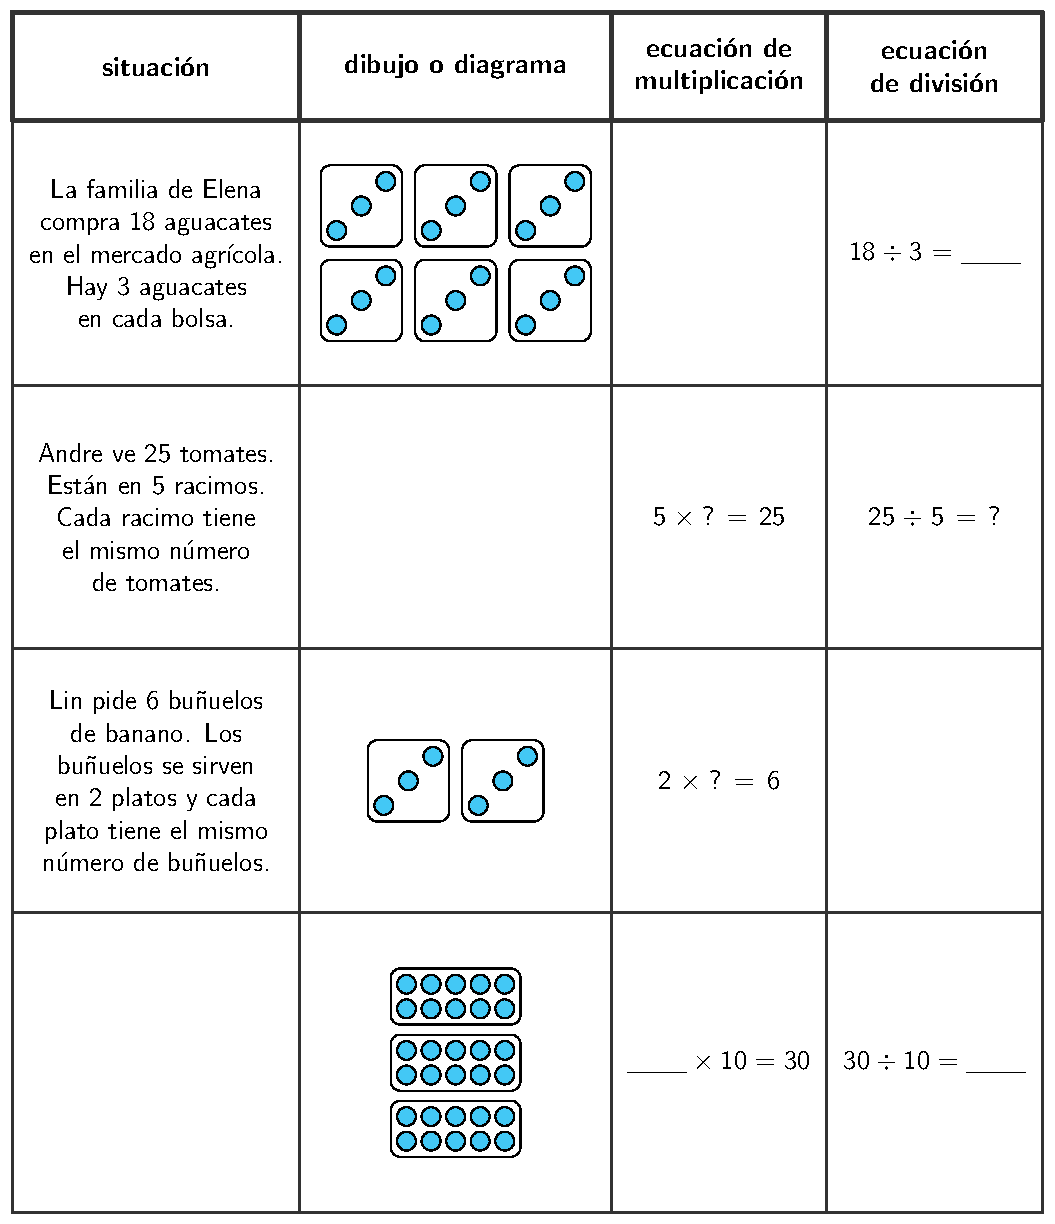
\includegraphics[max width=\linewidth, center]{external/tikz-source/enElMercadoAgricola-blm-tab.pdf}
\end{image}%
\end{activity}%
\end{subsubsectionptx}
%
%
\typeout{************************************************}
\typeout{Preguntas de comprensión  Actividad de cierre}
\typeout{************************************************}
%
\begin{reading-questions-subsubsection}{Preguntas de comprensión}{Actividad de cierre}{}{Actividad de cierre}{}{}{lec-divisionComoFactorDesconocido-cool}
\begin{project}{Actividad de cierre}{Muffins en cajas.}{cool-muffinsEnCajas}%
Hay 30 \emph{muffins} y varias cajas para la feria de pastelería. En cada caja hay 6 \emph{muffins}. ¿Cuántas cajas hay?%
\begin{sidebyside}{2}{0.05}{0.05}{0.1}%
\begin{sbspanel}{0.4}%
Tyler escribió dos ecuaciones para este problema.%
\end{sbspanel}%
\begin{sbspanel}{0.4}%
\(\underline{\hspace{1 cm}} \times 6 = 30\)%
\par
\(30 \div 6 = \underline{\hspace{1 cm}}\)%
\end{sbspanel}%
\end{sidebyside}%
\par
Él dice que en cada espacio en blanco va el mismo número, aunque una ecuación es de multiplicación y la otra es de división. ¿Tiene razón? Explica o muestra tu razonamiento.%
\begin{image}{0}{1}{0}{}%

\includegraphics[max width=\linewidth, center]{external/whitespace-tikz/2cm.pdf}
\end{image}%
\end{project}%
\end{reading-questions-subsubsection}
\end{subsectionptx}
%
%
\typeout{************************************************}
\typeout{Subsección  Lección 7 -~Relacionemos multiplicación y división}
\typeout{************************************************}
%
\begin{subsectionptx}{Subsección}{Lección 7 -~Relacionemos multiplicación y división}{}{Lección 7}{}{}{lec-relacionarMultiplicacionYDivision}
%
%
\typeout{************************************************}
\typeout{Subsubsección  Actividad 1}
\typeout{************************************************}
%
\clearpage
\begin{subsubsectionptx}{Subsubsección}{Actividad 1}{}{Actividad 1}{}{}{lec-relacionarMultiplicacionYDivision-act1}
\begin{activity}{Actividad}{Mesa redonda de división.}{act-mesaRedondaDeDivision}%
En esta tabla hay 4 recuadros. Tu profesor te pedirá que dibujes o escribas algo en cada uno.%
\par
Después de trabajar en cada recuadro, haz una pausa y espera que el profesor te dé las instrucciones para el siguiente recuadro.%
%
\begin{enumerate}
\item{}Dibuja grupos iguales en el recuadro 1 de tu hoja de registro.%
\item{}En el recuadro 2 de la hoja que acabaste de recibir, escribe una descripción de una situación de división que corresponda al dibujo.%
\item{}En el recuadro 3 de la hoja que acabas de recibir, escribe una ecuación de multiplicación que corresponda al dibujo y a la situación de división. Usa un símbolo para representar la cantidad desconocida.%
\item{}En el recuadro 4 de la hoja que acabas de recibir, escribe una ecuación de división que corresponda al dibujo, a la situación de división y a la ecuación de multiplicación. Usa un símbolo para representar la cantidad desconocida.%
\end{enumerate}
\begin{image}{0}{1}{0}{}%
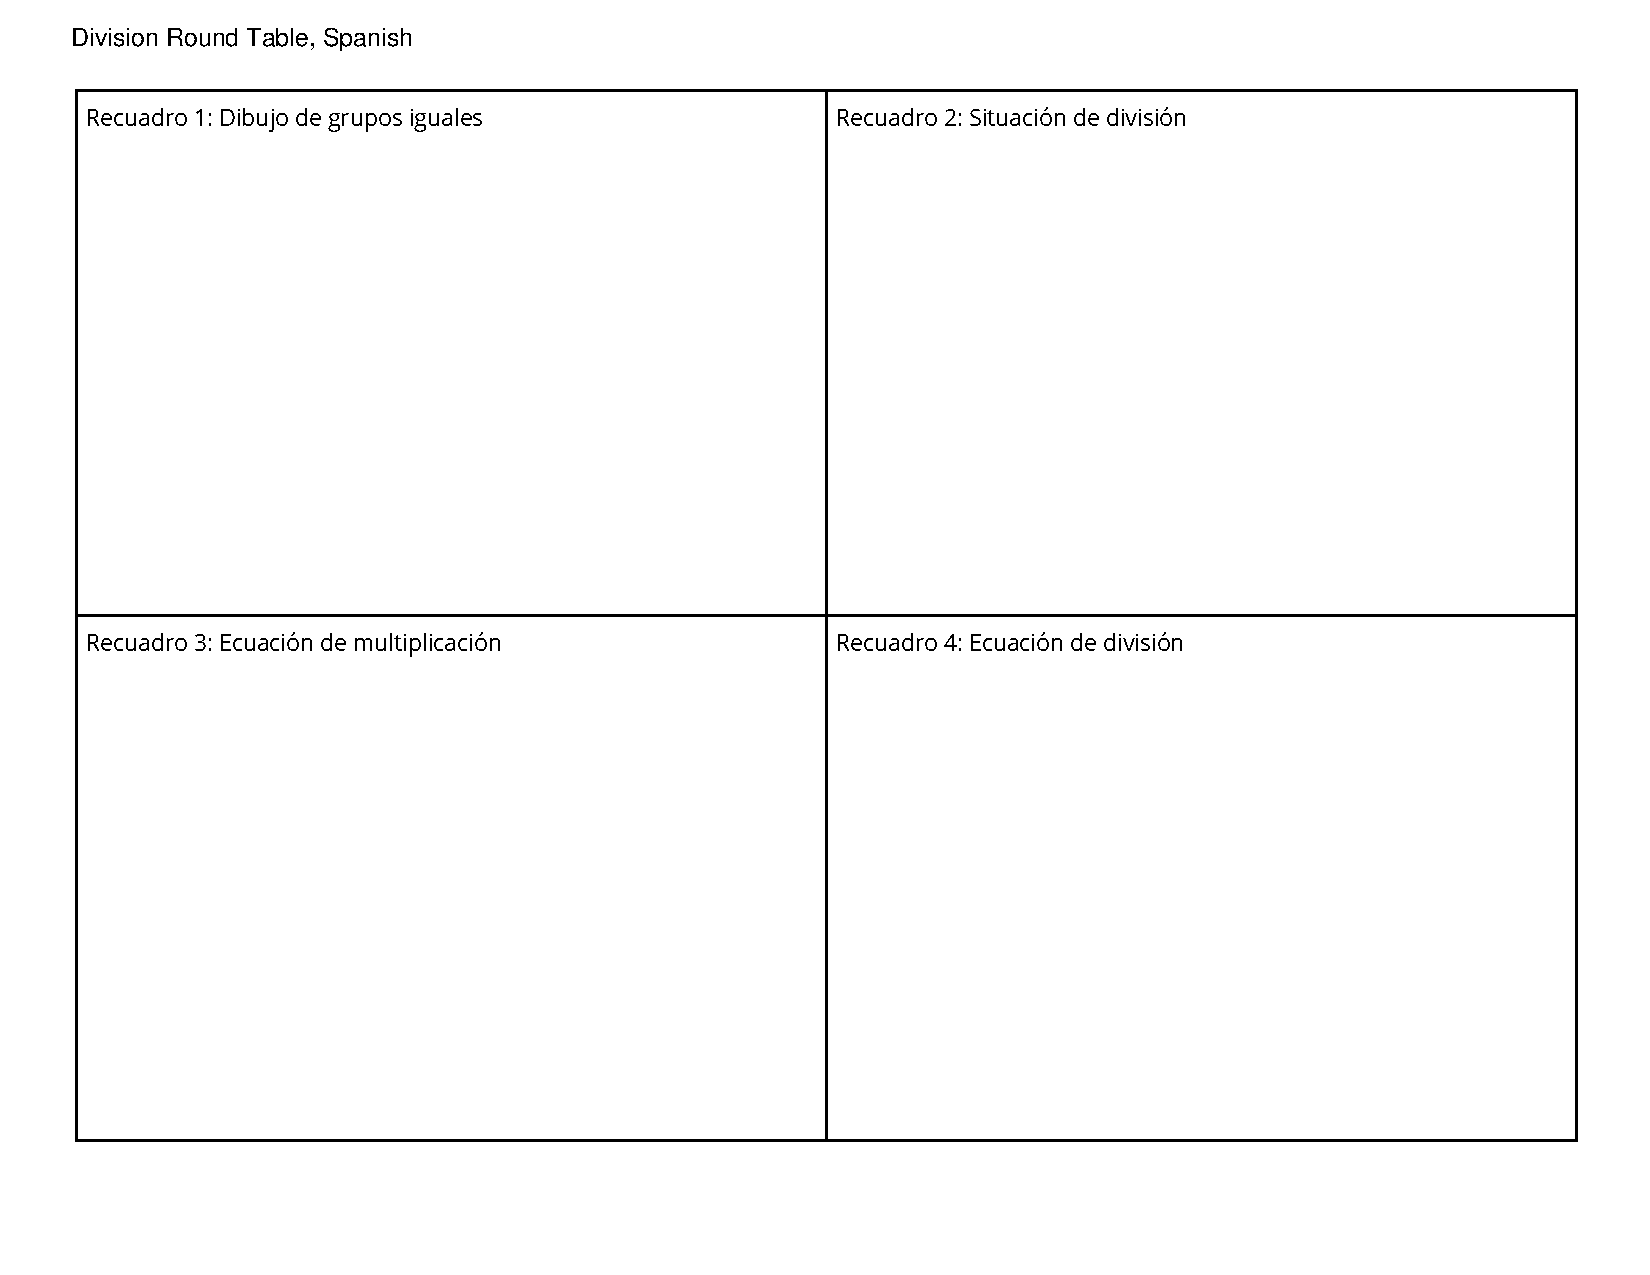
\includegraphics[trim=20 20 20 30, clip, width=1.5\linewidth,angle=90,origin=c]{external/blm/pdf-source/mesa-redonda-de-division.pdf}
\end{image}%
\end{activity}%
\end{subsubsectionptx}
%
%
\typeout{************************************************}
\typeout{Subsubsección  Actividad 2}
\typeout{************************************************}
%
\begin{subsubsectionptx}{Subsubsección}{Actividad 2}{}{Actividad 2}{}{}{lec-relacionarMultiplicacionYDivision-act2}
\begin{activity}{Actividad}{Grupos de útiles escolares.}{act-gruposUtilesEscolares}%
En cada situación:%
\par
(a) Escribe una ecuación que represente la situación. Usa un símbolo para representar la cantidad desconocida.%
\par
(b) Resuelve el problema y encuentra el número desconocido de la ecuación. Prepárate para explicar tu razonamiento.%
%
\begin{enumerate}
\item{}Kiran tenía 32 clips. Le dio 4 clips a cada estudiante. ¿Cuántos estudiantes recibieron clips?%
%
\begin{enumerate}
\item{}Ecuación:\fillintext{10}%
\item{}
\begin{image}{0}{1}{0}{}%
\includegraphics[max width=\linewidth, center]{external/whitespace-tikz/3cm.pdf}
\end{image}%
%
\end{enumerate}
\item{}Hay 28 libros en 4 pilas. Si cada pila tiene la misma cantidad de libros, ¿cuántos libros hay en cada pila?%
%
\begin{enumerate}
\item{}Ecuación:\fillintext{10}%
\item{}
\begin{image}{0}{1}{0}{}%
\includegraphics[max width=\linewidth, center]{external/whitespace-tikz/3cm.pdf}
\end{image}%
%
\end{enumerate}
\item{}Hay 6 cajas. En cada caja hay 8 borradores. ¿Cuántos borradores hay?%
%
\begin{enumerate}
\item{}Ecuación:\fillintext{10}%
\item{}
\begin{image}{0}{1}{0}{}%
\includegraphics[max width=\linewidth, center]{external/whitespace-tikz/2cm.pdf}
\end{image}%
%
\end{enumerate}
\item{}Lin tenía 36 notas adhesivas y varios cuadernos. Ella puso 6 notas adhesivas en cada cuaderno. ¿En cuántos cuadernos puso notas adhesivas?%
%
\begin{enumerate}
\item{}Ecuación:\fillintext{10}%
\item{}
\begin{image}{0}{1}{0}{}%
\includegraphics[max width=\linewidth, center]{external/whitespace-tikz/3cm.pdf}
\end{image}%
%
\end{enumerate}
\end{enumerate}
\end{activity}%
\end{subsubsectionptx}
%
%
\typeout{************************************************}
\typeout{Preguntas de comprensión  Actividad de cierre}
\typeout{************************************************}
%
\begin{reading-questions-subsubsection}{Preguntas de comprensión}{Actividad de cierre}{}{Actividad de cierre}{}{}{lec-relacionarMultiplicacionYDivision-cool}
\begin{project}{Actividad de cierre}{Rosas para compartir.}{cool-rosasParaCompartir}%
Clare tiene 14 rosas. Quiere darle 2 rosas a cada una de sus profesoras. ¿A cuántas profesoras les puede dar rosas?%
\par
Escribe una ecuación de multiplicación y una ecuación de división que representen la situación. Usa símbolos para representar los números desconocidos y explica tu razonamiento.%
\begin{image}{0}{1}{0}{}%
\includegraphics[max width=\linewidth, center]{external/whitespace-tikz/4cm.pdf}
\end{image}%
\end{project}%
\end{reading-questions-subsubsection}
\end{subsectionptx}
%
%
\typeout{************************************************}
\typeout{Subsección  Lección 8 -~Relacionemos cocientes con productos que nos sabemos}
\typeout{************************************************}
%
\begin{subsectionptx}{Subsección}{Lección 8 -~Relacionemos cocientes con productos que nos sabemos}{}{Lección 8}{}{}{lec-relCocientesProductos}
%
%
\typeout{************************************************}
\typeout{Subsubsección  Actividad 1}
\typeout{************************************************}
%
\clearpage
\begin{subsubsectionptx}{Subsubsección}{Actividad 1}{}{Actividad 1}{}{}{lec-relCocientesProductos-act1}
\begin{activity}{Actividad}{Clasificación de tarjetas: Multiplicación.}{act-clasificacionDeTarjetas-multiplicacion}%
Hazle preguntas a tu compañero sobre sus hechos de multiplicación. Clasifica los hechos de tu compañero en una de estas columnas:%
\begin{image}{0}{1}{0}{}%
\includegraphics[max width=\linewidth, center]{external/tikz-source/clasificacionTarjetas-mult-paraBLM.pdf}
\end{image}%
Anota cinco expresiones de multiplicación que vas a practicar.%
%
\begin{enumerate}
\item{}\vspace{0.5cm}
\item{}\vspace{0.5cm}%
\item{}\vspace{0.5cm}%
\item{}\vspace{0.5cm}%
\item{}\vspace{0.5cm}%
\end{enumerate}
%
\end{activity}%
\cleardoublepage
Tarjetas para recortar:
\par
\includegraphics[page=1, trim=70 80 80 100,clip, width=1.05\linewidth]{external/blm/tikz-source/clasificacionTarjetas-multiplicacion-blm.pdf}

\cleardoublepage
Más tarjetas para recortar:
\par
\includegraphics[page=2, trim=70 80 80 100,clip, width=1.05\linewidth]{external/blm/tikz-source/clasificacionTarjetas-multiplicacion-blm.pdf}
\par
\cleardoublepage
\end{subsubsectionptx}
%
%
\typeout{************************************************}
\typeout{Subsubsección  Actividad 2}
\typeout{************************************************}
%
\begin{subsubsectionptx}{Subsubsección}{Actividad 2}{}{Actividad 2}{}{}{lec-relCocientesProductos-act2}
\begin{activity}{Actividad}{Si sé que \textellipsis{}, entonces sé que \textellipsis{}.}{act-siSeQueEntoncesSeQue}%
Si sé que \(4 \times 5 = 20\), entonces sé que \fillintext{10}.%
%
\begin{enumerate}
\item{}Coloquen las tarjetas de hechos de multiplicación en un montón, boca abajo.%
\item{}Por turnos, tomen una tarjeta de hechos de multiplicación.%
\item{}Usen el hecho de multiplicación de la tarjeta para escribir una ecuación de multiplicación en la columna “Si sé que \textellipsis{}”%
\item{}Después, anoten las ecuaciones de división relacionadas en la columna “Entonces sé que   \textellipsis{}”%
\end{enumerate}
\begin{image}{0}{1}{0}{}%
\includegraphics[max width=\linewidth, center]{external/tikz-source/siSeQueEntoncesSeQue-tab-libroTrabajo.pdf}
\end{image}%
\end{activity}%
\end{subsubsectionptx}
%
%
\typeout{************************************************}
\typeout{Preguntas de comprensión  Actividad de cierre}
\typeout{************************************************}
%
\begin{reading-questions-subsubsection}{Preguntas de comprensión}{Actividad de cierre}{}{Actividad de cierre}{}{}{lec-relCocientesProductos-cool}
\begin{project}{Actividad de cierre}{Hechos de multiplicación y de división.}{cool-hechosMultiplicacionDivision}%
Piensa en los hechos de multiplicación que te sabes. ¿Cómo han cambiado desde el comienzo del año?%
\begin{image}{0}{1}{0}{}%
\includegraphics[max width=\linewidth, center]{external/whitespace-tikz/2cm.pdf}
\end{image}%
\end{project}%
\end{reading-questions-subsubsection}
\end{subsectionptx}
%
%
\typeout{************************************************}
\typeout{Subsección  Lección 9 -~Patrones en la tabla de multiplicar}
\typeout{************************************************}
%
\begin{subsectionptx}{Subsección}{Lección 9 -~Patrones en la tabla de multiplicar}{}{Lección 9}{}{}{lec-patronesTablaMultiplicar}
%
%
\typeout{************************************************}
\typeout{Subsubsección  Actividad 1}
\typeout{************************************************}
%
\begin{subsubsectionptx}{Subsubsección}{Actividad 1}{}{Actividad 1}{}{}{lec-patronesTablaMultiplicar-act1}
\begin{activity}{Actividad}{Productos en la tabla.}{act-productosTablaMultiplicar}%
Esta es una tabla de multiplicar que no se ha completado totalmente.%
\begin{image}{0}{1}{0}{}%
\includegraphics[max width=\linewidth, center]{external/svg-source/tikz-file-152978-scale13.pdf}
\end{image}%
%
\begin{enumerate}
\item{}Usa los productos de la tabla para ayudarte a encontrar los números que deberían ir en lugar de las letras de la A a la G. Prepárate para explicar tu razonamiento.%
\item{}Encuentra los números que deberían ir en otras tres casillas vacías de la tabla. Usa:%
%
\begin{enumerate}
\item{}7 como un factor%
\item{}9 como un factor%
\item{}10 como un factor%
\end{enumerate}
Prepárate para explicar tu razonamiento.%
\begin{image}{0}{1}{0}{}%
\includegraphics[max width=\linewidth, center]{external/whitespace-tikz/3cm.pdf}
\end{image}%
\end{enumerate}
\end{activity}%
\end{subsubsectionptx}
%
%
\typeout{************************************************}
\typeout{Subsubsección  Actividad 2}
\typeout{************************************************}
%
\begin{subsubsectionptx}{Subsubsección}{Actividad 2}{}{Actividad 2}{}{}{lec-patronesTablaMultiplicar-act2}
\begin{activity}{Actividad}{Si sé que \textellipsis{}, entonces sé que \textellipsis{}: Multiplicación.}{act-siSeQueEntoncesSeQueMult}%
%
\begin{enumerate}
\item{}En cada fila, escribe al menos dos hechos de multiplicación que puedes descifrar porque conoces el hecho de multiplicación dado en la columna de la izquierda. Prepárate para compartir tu razonamiento.%
\begin{image}{0}{1}{0}{}%
\includegraphics[max width=\linewidth, center]{external/tikz-source/siSeQueEntoncesSeQueMult-BLM-tab.pdf}
\end{image}%
\item{}Si te queda tiempo, completa el resto de la tabla de multiplicar. Usa los hechos de multiplicación que conoces para encontrar aquellos que no conoces.%
\end{enumerate}
\end{activity}%
\end{subsubsectionptx}
%
%
\typeout{************************************************}
\typeout{Preguntas de comprensión  Actividad de cierre}
\typeout{************************************************}
%
\begin{reading-questions-subsubsection}{Preguntas de comprensión}{Actividad de cierre}{}{Actividad de cierre}{}{}{lec-patronesTablaMultiplicar-cool}
\begin{project}{Actividad de cierre}{Encuentra el producto desconocido.}{cool-encuentraProductoDesconocido}%
¿Qué número debería ir en lugar del signo de interrogación? Explica o muestra tu razonamiento.%
\begin{image}{0}{1}{0}{}%
\includegraphics[max width=\linewidth]{external/svg-source/tikz-file-153040-scale13.pdf}
\end{image}%
% \begin{image}{0}{1}{0}{}%
% \includegraphics[max width=\linewidth, center]{external/whitespace-tikz/3cm.pdf}
% \end{image}%
\end{project}%
\end{reading-questions-subsubsection}
\end{subsectionptx}
%
%
\typeout{************************************************}
\typeout{Subsección  Lección 10 -~Exploremos estrategias de multiplicación con rectángulos}
\typeout{************************************************}
%
\begin{subsectionptx}{Subsección}{Lección 10 -~Exploremos estrategias de multiplicación con rectángulos}{}{Lección 10}{}{}{lec-estrategiasMultConRectangulos}
%
%
\typeout{************************************************}
\typeout{Subsubsección  Actividad 1}
\typeout{************************************************}
%
\begin{subsubsectionptx}{Subsubsección}{Actividad 1}{}{Actividad 1}{}{}{lec-estrategiasMultConRectangulos-act1}
\begin{activity}{Actividad}{De diagramas a expresiones.}{act-deDiagramasAExpresiones}%
%
\begin{enumerate}
\item{}Este es otro rectángulo.%
\begin{image}{0}{1}{0}{}%
\includegraphics[max width=\linewidth, center]{external/svg-source/tikz-file-153048.pdf}
\end{image}%
Podemos encontrar su área hallando \(4 \times 9\).%
%
\begin{enumerate}
\item{}Marca o colorea el rectángulo de una manera que te ayude a encontrar su área.%
\item{}Escribe una o más expresiones que representen lo que hiciste en el diagrama y muestra cómo encontraste el área.%
\end{enumerate}
\end{enumerate}
\end{activity}%
\end{subsubsectionptx}
%
%
\typeout{************************************************}
\typeout{Subsubsección  Actividad 2}
\typeout{************************************************}
%
\begin{subsubsectionptx}{Subsubsección}{Actividad 2}{}{Actividad 2}{}{}{lec-estrategiasMultConRectangulos-act2}
\begin{activity}{Actividad}{De expresiones a diagramas.}{act-deExpresionesADiagramas}%
\begin{sidebyside}{3}{0.0166666666666667}{0.0166666666666667}{0.0333333333333333}%
\begin{sbspanel}{0.3}%
Noah%
\par
\includegraphics[max width=\linewidth, center]{external/svg-source/tikz-file-153051.pdf}
%
\begin{equation*}
(5\times 3)+(2 \times 3)
\end{equation*}
%
\end{sbspanel}%
\begin{sbspanel}{0.3}%
Priya%
\par
\includegraphics[max width=\linewidth, center]{external/svg-source/tikz-file-153053.pdf}
%
\begin{equation*}
2 \times (2 \times 6)
\end{equation*}
%
\end{sbspanel}%
\begin{sbspanel}{0.3}%
Tyler%
\par
\includegraphics[max width=\linewidth, center]{external/svg-source/tikz-file-153054.pdf}
%
\begin{equation*}
(5 \times 8) + (3 \times 8)
\end{equation*}
%
\end{sbspanel}%
\end{sidebyside}%
\par
En cada rectángulo:%
%
\begin{enumerate}
\item{}Escribe los dos factores que se pueden multiplicar para encontrar su área.%
\item{}Marca o colorea cada rectángulo para mostrar la manera en la que cada estudiante vio el área. Prepárate para explicar tu razonamiento.%
\begin{image}{0}{1}{0}{}%
\includegraphics[max width=\linewidth, center]{external/whitespace-tikz/1cm.pdf}
\end{image}%
\end{enumerate}
\end{activity}%
\end{subsubsectionptx}
%
%
\typeout{************************************************}
\typeout{Preguntas de comprensión  Actividad de cierre}
\typeout{************************************************}
%
\begin{reading-questions-subsubsection}{Preguntas de comprensión}{Actividad de cierre}{}{Actividad de cierre}{}{}{lec-estrategiasMultConRectangulos-cool}
\begin{project}{Actividad de cierre}{Marca o colorea partes para encontrar el área.}{cool-marcaPartesParaEncontrarArea}%
\begin{sidebyside}{2}{0}{0}{0}%
\begin{sbspanel}{0.6}%
El área de este rectángulo se puede encontrar hallando \(6 \times 7\).%
%
\begin{enumerate}[label={(\alph*)}]
\item{}Marca o colorea el rectángulo para mostrar que podemos escribir \(2 \times (3 \times 7)\) o \((6 \times 5) + (6 \times 2)\) para encontrar su área.%
\item{}¿Cuál es el valor de \(6 \times 7\)? Explica o muestra tu razonamiento.%
\end{enumerate}
\end{sbspanel}%
\begin{sbspanel}{0.4}%
\includegraphics[scale=1.4, max width=\linewidth, center]{external/svg-source/tikz-file-153042.pdf}
\end{sbspanel}%
\end{sidebyside}%
% \begin{image}{0}{1}{0}{}%
% \includegraphics[max width=\linewidth, center]{external/whitespace-tikz/3cm.pdf}
% \end{image}%
\end{project}%
\end{reading-questions-subsubsection}
\end{subsectionptx}
%
%
\typeout{************************************************}
\typeout{Subsección  Lección 11 -~Estrategias de multiplicación para rectángulos sin cuadrícula}
\typeout{************************************************}
%
\begin{subsectionptx}{Subsección}{Lección 11 -~Estrategias de multiplicación para rectángulos sin cuadrícula}{}{Lección 11}{}{}{lec-estrategiasMultRectangulosSinCuadricula}
%
%
\typeout{************************************************}
\typeout{Subsubsección  Actividad 1}
\typeout{************************************************}
%
\begin{subsubsectionptx}{Subsubsección}{Actividad 1}{}{Actividad 1}{}{}{gra3-uni4-secB-lec11-act1}
\begin{activity}{Actividad}{Marca y después expresa.}{act-marcaDespuesExpresa}%
En cada caso:%
%
\begin{itemize}[label=\textbullet]
\item{}Marca o colorea cada rectángulo para mostrar una estrategia que ayude a encontrar su área.%
\item{}Escribe una o más expresiones que representen cómo encuentras el área.%
\end{itemize}
\begin{sidebyside}{3}{0}{0}{0}%
\begin{sbspanel}{0.391}%
A%
\par
\includegraphics[max width=\linewidth, center]{external/svg-source/tikz-file-153084.pdf}
\end{sbspanel}%
\begin{sbspanel}{0.261}%
B%
\par
\includegraphics[max width=\linewidth, center]{external/svg-source/tikz-file-153085.pdf}
\end{sbspanel}%
\begin{sbspanel}{0.348}%
C%
\par
\includegraphics[max width=\linewidth, center]{external/svg-source/tikz-file-153086.pdf}
\end{sbspanel}%
\end{sidebyside}%
\begin{image}{0}{1}{0}{}%
\includegraphics[max width=\linewidth, center]{external/whitespace-tikz/2cm.pdf}
\end{image}%
\end{activity}%
\end{subsubsectionptx}
%
%
\typeout{************************************************}
\typeout{Subsubsección  Actividad 2}
\typeout{************************************************}
%
\begin{subsubsectionptx}{Subsubsección}{Actividad 2}{}{Actividad 2}{}{}{gra3-uni4-secB-lec11-act2}
\begin{activity}{Actividad}{Clasificación de tarjetas: Expresiones diferentes, mismo rectángulo.}{act-clasificacionDeTarjetas-expresionesMultiplicacionRectangulos}%
Las tarjetas para recortar tienen expresiones que representan áreas de rectángulos.%
\par
Clasifica las expresiones en grupos de manera que las expresiones de cada grupo representen el área del mismo rectángulo. Prepárate para explicar tu razonamiento.%
\par
Si te ayuda, puedes dibujar rectángulos.%
\cleardoublepage
\begin{image}{0}{1}{0}{}%
\includegraphics[max width=\linewidth, center]{external/blm/tikz-source/clasificacionTarjetas-expresionesDiferentesMismoRect-tarjetas.pdf}
\end{image}%
%
\end{activity}%
\end{subsubsectionptx}
%
%
\typeout{************************************************}
\typeout{Preguntas de comprensión  Actividad de cierre}
\typeout{************************************************}
%
\begin{reading-questions-subsubsection}{Preguntas de comprensión}{Actividad de cierre}{}{Actividad de cierre}{}{}{gra3-uni4-secB-lec11-cool}
\begin{project}{Actividad de cierre}{Expresiones para un rectángulo.}{cool-expresionesParaRectangulo}%
\begin{sidebyside}{2}{0}{0}{0}%
\begin{sbspanel}{0.6}%
%
\begin{enumerate}[label={(\alph*)}]
\item{}Marca o colorea este rectángulo para mostrar una estrategia que ayude a encontrar su área.%
\item{}Escribe una o más expresiones que representen cómo encuentras el área.%
\end{enumerate}
\end{sbspanel}%
\begin{sbspanel}{0.4}%
\includegraphics[max width=\linewidth, center]{external/svg-source/tikz-file-158678-scale13.pdf}
\end{sbspanel}%
\end{sidebyside}%
\begin{image}{0}{1}{0}{}%
\includegraphics[max width=\linewidth, center]{external/whitespace-tikz/2cm.pdf}
\end{image}%
\end{project}%
\end{reading-questions-subsubsection}
\end{subsectionptx}
%
%
\typeout{************************************************}
\typeout{Ejercicios  Problemas de práctica de la sección B}
\typeout{************************************************}
%
\begin{exercises-subsection}{Ejercicios}{Problemas de práctica de la sección B}{}{Problemas de práctica}{}{}{gra3-uni4-secB-ProblemasPractica}
\begin{divisionexercise}{1}{}{}{gra3-uni4-secB-ProblemasPractica-3}%
Hay 35 libros en la estantería. Hay 7 libros en cada estante. ¿Cuántos estantes hay? Explica de qué manera las ecuaciones \(35 \div 7 = {?}\) y \({?} \times 7 = 35\) representan la situación.%
\begin{image}{0}{1}{0}{}%
\includegraphics[max width=\linewidth, center]{external/whitespace-tikz/2cm.pdf}
\end{image}%
\end{divisionexercise}%
\begin{divisionexercise}{2}{}{}{gra3-uni4-secB-ProblemasPractica-4}%
Hay 24 huevos en la caja. Hay 6 en cada fila. ¿Cuántas filas de huevos hay?%
\par
Escribe una ecuación que represente la situación. Usa un símbolo para representar el número desconocido. Después, contesta la pregunta.%
\begin{image}{0}{1}{0}{}%
\includegraphics[max width=\linewidth, center]{external/whitespace-tikz/2cm.pdf}
\end{image}%
\end{divisionexercise}%
\begin{divisionexercise}{3}{}{}{gra3-uni4-secB-ProblemasPractica-5}%
En cada caso, escribe un hecho de división que te sepas y que esté relacionado con la ecuación de multiplicación.%
%
\begin{enumerate}[label={(\alph*)}]
\item{}\(\displaystyle 8 \times 5 = 40\)%
\begin{image}{0}{1}{0}{}%
\includegraphics[max width=\linewidth, center]{external/whitespace-tikz/1cm.pdf}
\end{image}%
\item{}\(\displaystyle 2 \times 9 = 18\)%
\begin{image}{0}{1}{0}{}%
\includegraphics[max width=\linewidth, center]{external/whitespace-tikz/1cm.pdf}
\end{image}%
\end{enumerate}
\end{divisionexercise}%
\begin{divisionexercise}{4}{}{}{gra3-uni4-secB-ProblemasPractica-6}%
Lin sabe que \(8 \times 5 = 40\). Explica cómo puede usar este hecho para encontrar \(8 \times 4\).%
\begin{image}{0}{1}{0}{}%
\includegraphics[max width=\linewidth, center]{external/whitespace-tikz/2cm.pdf}
\end{image}%
\end{divisionexercise}%
\begin{divisionexercise}{5}{}{}{gra3-uni4-secB-ProblemasPractica-7}%
%
\vspace{-1.3\baselineskip}
\begin{enumerate}[label={(\alph*)}]
\item{}Resalta partes del diagrama para mostrar la expresión \((5 \times 7) + (2 \times 7)\)%
\begin{image}{0}{1}{0}{}%
\includegraphics[max width=\linewidth, center]{external/svg-source/tikz-file-151677-scale13.pdf}
\end{image}%
\item{}Explica cómo podrías usar el diagrama para calcular \(7\times 7\).%
\begin{image}{0}{1}{0}{}%
\includegraphics[max width=\linewidth, center]{external/whitespace-tikz/2cm.pdf}
\end{image}%
\end{enumerate}
\end{divisionexercise}%
\begin{divisionexercise}{6}{}{}{gra3-uni4-secB-ProblemasPractica-8}%
\vspace{-2.6ex}
\begin{sidebyside}{2}{0}{0}{0}%
\begin{sbspanel}{0.6}%
Marca o colorea el rectángulo para mostrar una estrategia que te permita encontrar su área. Después, explica cómo usar el diagrama para encontrar el área.%
\end{sbspanel}%
\begin{sbspanel}{0.4}%
\includegraphics[scale=1.2, max width=\linewidth, center]{external/svg-source/tikz-file-159147-scale13.pdf}
\end{sbspanel}%
\end{sidebyside}%
\end{divisionexercise}%
\clearpage
\begin{divisionexercise}{7}{Exploración.}{}{gra3-uni4-secB-ProblemasPractica-9}%
Noah encuentra \(9 \times 8\) calculando \((10 \times 8) - (1 \times 8)\).%
%
\begin{enumerate}[label={(\alph*)}]
\item{}Haz un dibujo que muestre por qué funciona el cálculo de Noah.%
\begin{image}{0}{1}{0}{}%
\includegraphics[max width=\linewidth, center]{external/whitespace-tikz/6cm.pdf}
\end{image}%
\item{}Usa el método de Noah para calcular \(9\times 8\).%
\begin{image}{0}{1}{0}{}%
\includegraphics[max width=\linewidth, center]{external/whitespace-tikz/3cm.pdf}
\end{image}%
\end{enumerate}
\end{divisionexercise}%
\end{exercises-subsection}
%
%
\end{document}
